% GNN-Based Lung Nodule Malignancy Classification Using Multi-Modal Feature Embedding on CT Scans
% NeurIPS-style two-column research paper
% Authors: Harrison Lavins, Rensildi Kalanxhi, Swathi Gopal
% Compile with: pdflatex gnn_lung_nodule_classification.tex (twice for refs)

\documentclass[10pt,letterpaper,twocolumn]{article}

% --- Geometry: NeurIPS-like margins, adapted for two columns ---
\usepackage[letterpaper,
            left=0.75in, right=0.75in,
            top=1.0in, bottom=1.0in,
            columnsep=0.3in]{geometry}

% --- Fonts: Times-like, NeurIPS aesthetic ---
\usepackage[T1]{fontenc}
\usepackage[utf8]{inputenc}
\usepackage{mathptmx}
\usepackage{microtype}

% --- Math, graphics, tables ---
\usepackage{amsmath}
\usepackage{amssymb}
\usepackage{graphicx}
\graphicspath{{figures/}}
\usepackage{booktabs}
\usepackage{array}
\usepackage{multirow}
\usepackage{caption}
\captionsetup{font=small,labelfont=bf,labelsep=period}

% --- Hyperlinks (NeurIPS style: black text, no boxes) ---
\usepackage[hidelinks,colorlinks=true,
            citecolor=black,linkcolor=black,urlcolor=black]{hyperref}
\usepackage{url}

% --- NeurIPS-style section headings ---
\usepackage{titlesec}
\titleformat{\section}{\normalfont\large\bfseries}{\thesection}{0.5em}{}
\titleformat{\subsection}{\normalfont\normalsize\bfseries}{\thesubsection}{0.5em}{}
\titleformat{\subsubsection}{\normalfont\normalsize\itshape}{\thesubsubsection}{0.5em}{}
\titlespacing*{\section}{0pt}{1.0\baselineskip}{0.4\baselineskip}
\titlespacing*{\subsection}{0pt}{0.7\baselineskip}{0.3\baselineskip}

% (Title is typeset manually inside \twocolumn[] so it spans both columns.)

% --- Equation, figure, and table numbering ---
\renewcommand{\theequation}{\arabic{equation}}
\renewcommand{\thefigure}{\arabic{figure}}
\renewcommand{\thetable}{\arabic{table}}

% --- Spacing tweaks ---
\setlength{\parskip}{0.4em}
\setlength{\parindent}{0pt}

% =====================================================================
\begin{document}

% --- Single-column title block and abstract spanning both columns ---
\twocolumn[%
  \begin{center}
    {\LARGE\bfseries GNN-Based Lung Nodule Malignancy Classification\\
     Using Multi-Modal Feature Embedding on CT Scans \par}
    \vspace{0.9em}
    {\large Harrison Lavins\quad Rensildi Kalanxhi\quad Swathi Gopal \par}
    \vspace{0.3em}
    {\small\itshape CSC 7760, Deep Learning, April 2026 \par}
  \end{center}
  \vspace{0.8em}
\begin{center}
\begin{minipage}{0.92\textwidth}
\begin{center}\textbf{Abstract}\end{center}
\small
We investigate whether modeling inter-nodule similarity as a graph improves benign-versus-malignant lung-nodule classification on CT. A two-stage pipeline fuses three complementary per-nodule modalities, namely frozen 3D imaging features (Med3D ResNet-50 or FMCIB), embeddings of the eight LIDC-IDRI radiologist attributes, and a sinusoidal positional encoding of the nodule's spatial coordinates, into a 256-dimensional node feature. A two-layer Graph Convolutional Network (GCN) operating over a cohort-wide $k$-nearest-neighbor (KNN) similarity graph is benchmarked against a parameter-matched multilayer perceptron (MLP) under patient-level five-fold cross-validation on 1{,}128 labeled LIDC-IDRI nodules from 588 patients. Across four pre-registered experiments and one side study, we find that (i) the GCN does not beat the MLP under standard radiologist-consensus labels (AUC $0.949$ versus $0.968$, paired Wilcoxon $p=0.031$, MLP wins five of five folds; H1 rejected); (ii) graph-construction hyperparameters do not recover the gap, with smaller $k$ preferred but no cell beating the default at Bonferroni-corrected significance; (iii) the FMCIB foundation model substantially outperforms Med3D as the image encoder on image-only inputs ($+0.27$ AUC, five of five folds), but the advantage vanishes once attribute features are added because both encoders saturate at the attribute-driven ceiling; and (iv) a side-study evaluation against the 157-patient pathology-confirmed ground truth reveals a striking inversion in which the radiologist-consensus winner loses, FMCIB image-only is the best cell on biopsy and surgery labels (AUC $0.887$, 95\% CI $\lbrack 0.761, 0.982 \rbrack$), and the attribute branch actively degrades pathology AUC by approximately $0.16$ on FMCIB. Radiologist-consensus and pathology labels agree on only $67.5\%$ of the matched subset, providing a direct ceiling on label-leaky models. We conclude that the LIDC-IDRI attribute branch acts as a label shortcut rather than orthogonal clinical signal, and that graph-based similarity reasoning has not yet had a fair test on this dataset. Adopting FMCIB image-only features is recommended for cross-dataset generalization, where the attribute branch is unavailable.
\end{minipage}
\end{center}
\vspace{0.8em}
]

% =====================================================================
\section{Introduction}
\label{sec:intro}

Lung cancer is the leading cause of cancer-related mortality worldwide. Modern CT-based classifiers reach AUC $0.88$ to $0.96$ on the public LIDC-IDRI benchmark, but they treat each lung nodule as an independent classification target. Patients in real-world cohorts share recurring imaging patterns: morphologically similar nodules tend to share clinical outcomes, and a clinician examining a borderline case implicitly compares it against similar prior cases. This project asks whether such guilt-by-association reasoning can be operationalized inside a deep-learning pipeline. Specifically, we ask: does modeling inter-nodule similarity as a graph improve malignancy classification compared to classifying each nodule independently?

The methodological contribution is a side-by-side, parameter-matched comparison of a two-layer Graph Convolutional Network against a parameter-matched MLP on a shared multi-modal feature representation. To prevent confounding from the choice of image encoder we test two pretrained 3D extractors: Med3D ResNet-50 (Chen et al.\ 2019) and the FMCIB foundation model (Pai et al.\ 2024). To distinguish image signal from radiologist-attribute leakage we ablate the input modality. To check whether the comparison is being made on a meaningful ground truth at all, we re-evaluate against the 157-patient pathology-confirmed subset of LIDC-IDRI.

Five experiments are reported in this paper. Experiment 1 is the GCN versus MLP baseline under the full multi-modal feature configuration. Experiment 2 is a graph-construction ablation over $k \in \{5, 10, 15, 20\}$ and similarity metric $\in \{\text{cosine}, \text{euclidean}\}$. Experiment 3 is a feature-modality by encoder ablation arranged as a three-by-two grid. Experiment 3.1 is a pathology-subset re-evaluation of every Experiment-3 cell against biopsy and surgery ground truth. Experiment 4 is preliminary work on cross-dataset generalization to LUNA25.

The paper proceeds as follows. Section~\ref{sec:background} reviews technical background. Section~\ref{sec:related} surveys prior progress. Section~\ref{sec:methodology} describes the architecture. Section~\ref{sec:experiments} defines each experiment, its dataset use, and its protocol. Section~\ref{sec:results} presents empirical results and a cross-experiment discussion. Section~\ref{sec:contributions} enumerates contributions. Section~\ref{sec:conclusion} concludes; Section~\ref{sec:future} outlines future work; Section~\ref{sec:references} lists references. Appendices A through G reproduce the full architecture diagrams and an additional pathology heatmap.

% =====================================================================
\section{Background}
\label{sec:background}

\subsection{Lung-nodule classification on CT}

Pulmonary nodules, small ($<30$~mm) opacities visible on chest CT, are the principal radiological finding triaged for possible lung malignancy. Computer-aided diagnosis on CT has progressed from hand-engineered radiomics through 2D and 3D convolutional neural networks. The modern public benchmark is the Lung Image Database Consortium / Image Database Resource Initiative (LIDC-IDRI) collection, whose protocol calls for up to four blinded thoracic radiologists per scan to mark and rate every nodule of at least 3~mm.

\subsection{Convolutional networks and ResNet}

Convolutional Neural Networks extract translation-equivariant local features and are the default architecture for medical image analysis. The ResNet family (He et al.\ 2016) addresses vanishing-gradient pathologies via skip connections that allow the optimizer to fit residual functions. In 3D medical imaging, the same principle ports directly to 3D convolutions; 3D ResNet-18, 3D ResNet-50, and their wider variants serve as standard frozen feature extractors for nodule patches.

\subsection{Graph neural networks and the GCN}

Graph Neural Networks are the family of architectures designed for graph-structured inputs, namely sets of nodes connected by edges. The Graph Convolutional Network (GCN, Kipf and Welling 2017) is the canonical instance: each layer computes a normalized weighted average of every node's neighbors, applies a learned linear map, and then a nonlinearity:
\begin{equation}
\label{eq:gcn-update}
H^{(l+1)} = \sigma\!\left(\tilde{D}^{-1/2}\tilde{A}\,\tilde{D}^{-1/2}\,H^{(l)}\,W^{(l)}\right),
\end{equation}
where $\tilde{A} = A + I$ adds self-loops and $\tilde{D}$ is its degree matrix. Two layers give a two-hop receptive field, the standard depth on small graphs since deeper stacks suffer over-smoothing as node representations collapse toward the graph mean. In our setup, nodes are nodules and edges encode inter-nodule similarity; the GCN refines each nodule's representation using the representations of its $k$ nearest neighbors in the shared 256-dimensional feature space.

\subsection{Foundation models in medical imaging}

Foundation models are large-scale pretrained networks released as frozen feature extractors and as fine-tuning starting points for downstream tasks. Two relevant 3D backbones inform this project. Med3D (Chen et al.\ 2019) is a 3D ResNet pretrained on 23 medical segmentation datasets via supervised multi-task learning; we use the 23-dataset ResNet-50 weights as the project's reported image baseline because the closest prior GCN-on-LIDC work (Ma et al.\ 2023) reports against an encoder of this kind. FMCIB (Foundation Model for Cancer Imaging Biomarkers, Pai et al.\ 2024, \textit{Nature Machine Intelligence}) is a wide 3D ResNet-50 (widen factor of two) pretrained with SimCLR contrastive self-supervised learning on roughly 11{,}000 lesion-containing CT scans across multiple tumor types and institutions. The contrastive objective explicitly clusters similar lesion patches in feature space, which is precisely the inductive bias a downstream similarity-graph GNN benefits from.

\subsection{Datasets}

LIDC-IDRI ($1{,}010$ patients, $1{,}308$ CT studies, approximately $7{,}371$ nodules of at least 3~mm with up to four radiologist ratings each) provides our primary training and within-dataset evaluation set. A subset of 157 patients carries pathology-confirmed diagnoses (biopsy, surgical resection, or two-year radiological follow-up), distributed via the TCIA \texttt{tcia-diagnosis-data-2012-04-20.xls} spreadsheet. LUNA25 ($4{,}096$ CT exams, $6{,}163$ nodules from the U.S.\ National Lung Screening Trial, MICCAI 2025 release) provides our planned cross-dataset evaluation set. Nodule-level binary malignancy labels in LUNA25 come from clinical follow-up rather than radiologist consensus.

% =====================================================================
\section{Previous Progress and Related Work}
\label{sec:related}

CT-based lung-nodule classifiers have improved steadily over the last decade, with reported LIDC-IDRI AUCs in the $0.88$ to $0.96$ range. Most published methods share two limitations from our perspective. First, they classify each nodule independently. Even multi-task networks that reason about shape and texture jointly produce a single per-nodule prediction with no architectural mechanism for the model to relate one case to another. Patient-similarity graph methods exist in adjacent applications such as cancer subtyping and prognosis prediction, but had not previously been applied to lung-nodule malignancy classification on CT. Second, the most common LIDC-IDRI evaluation protocol uses radiologist-consensus labels (mean malignancy rating across up to four readers, then binarized) and reports a single dataset-level AUC. As Section~\ref{sec:results} shows, that protocol can mask a substantial gap between fitting radiologist opinion and learning real malignancy signal.

The closest prior work is Ma et al.\ (2023), \textit{BMC Pulmonary Medicine} 23:462, whose LIDC-IDRI GCN reaches AUC $0.9629$ by using GCN layers for cross-CNN feature fusion. Their setup concatenates features from multiple CNNs and applies graph convolutions over the resulting feature graph. Our setup is architecturally distinct: we use GCN layers for node classification on a nodule-similarity graph, where nodes are nodules and edges are inter-nodule $k$-nearest-neighbor connections. Both architectures are GCNs in the Kipf-Welling sense, but they operate on different graphs and answer different questions. To our knowledge, the present project is the first systematic comparison of Med3D and FMCIB encoders on LIDC-IDRI nodule classification and the first node-classification GCN evaluated on the inter-nodule similarity graph for this task.

% =====================================================================
\section{Methodology}
\label{sec:methodology}

The architecture is a two-stage pipeline. Stage~1 is held frozen at inference; only Stage~2 is trained end-to-end. Appendix~A reproduces the full pipeline diagram, and Appendices~B and~C give the per-head detail.

\subsection{Stage 1: multi-modal feature fusion (frozen)}

Each nodule is represented by a 256-dimensional feature vector formed by concatenating three branches and projecting through a LayerNorm and Linear layer. The image branch extracts a $48^3$-voxel patch (Med3D) or $50^3$-voxel patch (FMCIB) around the nodule's centroid in the resampled isotropic $1$~mm$^3$ volume. Patches are HU-clipped to $[-1000, 400]$ and normalized to $[0, 1]$ for Med3D, or HU-normalized as $(\mathrm{HU} + 1024)/3072$ for FMCIB. Each patch is passed through the frozen 3D ResNet, producing a globally-pooled feature vector of dimension $2048$ for Med3D or $4096$ for FMCIB; a trainable linear projection reduces this to 256 dimensions. The clinical branch looks up the eight LIDC-IDRI radiologist attribute ratings (subtlety, internal structure, calcification, sphericity, margin, lobulation, spiculation, and texture) in eight per-attribute embedding tables of width eight, concatenated into a 64-dimensional vector. The spatial branch encodes the nodule's centroid coordinates $(x, y, z)$ in millimeters using sinusoidal positional encoding (16 dimensions per axis times three axes, yielding 48 dimensions) in the Transformer style. The three branches are concatenated, LayerNorm-ed, and projected through a final linear map to a 256-dimensional unified node feature. Critically, the malignancy label is not part of any branch: Stage~1 produces inputs to a classifier that has not yet seen the label.

\subsection{Stage 2: trainable node-classification head}

Two heads are compared with all hyperparameters held identical except for the architecture itself. The GCN head (treatment) consists of two GCNConv layers (Kipf and Welling 2017, via PyTorch Geometric) operating over a cohort-wide $k$-nearest-neighbor similarity graph in the 256-dimensional Stage-1 space, with default $k = 10$ and default cosine similarity. Each layer applies symmetric normalization with self-loops, ReLU activation, and dropout $p = 0.3$; a final linear layer maps the 64-dimensional output to two class logits. The MLP head (control) consists of three linear layers with ReLU and Dropout(0.3) between them, sized identically to the GCN's per-layer widths. The parameter count is matched within $\pm 20\%$, so any AUC delta cannot be explained by capacity differences. The MLP has no graph structure; each nodule is processed independently.

\subsection{Inductive graph construction}

A na\"ive cohort-wide KNN graph would produce a transductive leakage path under patient-level cross-validation, since validation nodules' features would influence training nodules' representations through KNN edges. To prevent this we use an inductive evaluation protocol. KNN edges are built over training-fold nodules only; at evaluation time, validation nodules are inserted into the graph as new nodes whose edges connect only to their $k$ nearest training neighbors; no validation-to-validation edges are ever created. We verified this setup by checking that no patient straddles train and validation in any fold (StratifiedGroupKFold with groups equal to the patient identifier).

\subsection{Training protocol}

We use the Adam optimizer with learning rate $1{\times}10^{-3}$ and weight decay $1{\times}10^{-4}$; weighted cross-entropy loss with per-fold inverse-frequency class weights to compensate for the approximately $71\%/29\%$ benign/malignant imbalance; and up to 100 epochs with patience-15 early stopping on validation AUC. The best checkpoint by validation AUC is retained. Cross-validation uses patient-level five-fold StratifiedGroupKFold (seed 42); per-fold validation malignant counts are 67, 77, 63, 62, and 54, all comfortably above the pre-registered minimum of 30. Reproducibility relies on globally-set torch and numpy seeds and \texttt{torch.backends.cudnn.deterministic = True}; per-cell seed reset is used in Experiments 2 and 3 so that the only cell-level variable is the architectural or feature-config knob being studied.

\subsection{Evaluation metrics}

Per fold we report AUC, AUPRC, sensitivity and specificity at the Youden-J optimal threshold (computed on training, applied to validation), Brier score, and a 10-bin reliability diagram. Across folds we compute the mean and standard deviation, plus paired Wilcoxon signed-rank tests for matched cell pairs. Bonferroni correction is applied across all simultaneous comparisons in Experiment 2. For Experiment 3.1 (pathology subset), the matched subset is small (40 nodules) so per-fold AUCs are often undefined; we report pooled AUC across folds with bootstrap $95\%$ confidence intervals from $1{,}000$ paired resamples.

% =====================================================================
\section{Experiments}
\label{sec:experiments}

\subsection{Datasets and preprocessing}

LIDC-IDRI is the primary dataset. After XML parsing, cross-reader clustering, malignancy binarization (mean rating $\le 2$ maps to benign; $\ge 4$ to malignant; the ambiguous middle band is excluded from training and evaluation), and patient-level deduplication, we obtain $1{,}128$ labeled nodules across 588 patients (805 benign, 323 malignant). The pathology-confirmed subset comprises 157 patients with biopsy, surgery, or two-year follow-up labels. LUNA25 ($4{,}096$ CT exams, $6{,}163$ NLST-derived nodules with clinical-follow-up binary labels, distributed via Zenodo under CC BY 4.0) is the cross-dataset evaluation set used in Experiment 4.

The preprocessing pipeline is implemented without \texttt{pylidc}. XML annotations are parsed with the Python standard library, with the malignancy rating tracked in a dedicated field separate from the eight feature-attribute fields, so that the Stage-1 fusion module cannot accidentally consume the label as a feature. DICOM series are loaded via \texttt{pydicom}, with slices ordered by physical Z (\texttt{ImagePositionPatient[2]}) so the loader is robust to vendors that reverse \texttt{InstanceNumber}; per-slice \texttt{RescaleSlope} and \texttt{RescaleIntercept} are applied to convert raw pixel intensities to Hounsfield Units. Cross-reader nodule clustering uses greedy centroid-distance matching at an 8~mm threshold, aggregating up to four radiologists' annotations of the same physical nodule. Patches are extracted at the encoder's expected size ($48^3$ voxels for Med3D, $50^3$ for FMCIB) centered on each nodule, and resampled to isotropic $1$~mm$^3$ before encoder inference. Patient-level five-fold StratifiedGroupKFold splits are committed under \texttt{data/splits/} and were verified for zero patient overlap before any training run.

\subsection{Experiment 1: GCN versus MLP baseline}

This experiment is the direct head-to-head test of whether graph structure improves malignancy classification when both heads see the same features. The pre-registered hypothesis (H1) states that the GCN macro-AUC exceeds the MLP macro-AUC by at least $0.01$, with paired Wilcoxon signed-rank $p < 0.05$ across the five CV folds. Stage~1 is fixed at the full multi-modal configuration (image, attributes, and spatial branches active); Stage~2 is either the two-layer GCN or the parameter-matched MLP. Optimizer, schedule, loss, and seeds are identical across the two arms.

\subsection{Experiment 2: graph-construction ablation}

This experiment asks whether different $(k, \text{metric})$ choices recover any of the GCN gap. Eight cells are evaluated: $k \in \{5, 10, 15, 20\}$ crossed with metric $\in \{\text{cosine}, \text{euclidean}\}$. The GCN architecture is fixed at Experiment 1's; only the KNN graph differs per cell. Per-cell seed reset isolates the graph effect from initialization noise. The decision rule treats the best cell as the new default if its improvement clears Bonferroni-corrected $p < 0.05$ against the $(10, \text{cosine})$ baseline; otherwise the default is retained.

\subsection{Experiment 3: feature-modality by encoder ablation}

This experiment disentangles the two remaining hypotheses left standing after Experiments 1 and 2: that the headline result was driven by attribute-branch label leakage, and that the Med3D image encoder was the bottleneck. We evaluate a three-by-two grid where the feature axis takes three levels (image only; image plus attributes; image plus attributes plus spatial) and the encoder axis takes two levels (Med3D ResNet-50 baseline; FMCIB follow-up). Stage~2 is held fixed at Experiment 1's GCN with $(k = 10, \text{cosine})$. Five folds times six cells equals 30 model trainings. Appendix~D reproduces the grid architecturally.

\subsection{Experiment 3.1: pathology-subset re-evaluation}

This side study re-evaluates every Experiment-3 cell against the biopsy and surgery ground truth in the TCIA pathology spreadsheet, rather than against radiologist-consensus labels. The matching strategy is conservative: per-nodule diagnoses from the spreadsheet are binarized ($1$ to benign; $\{2, 3\}$ to malignant; $0$ dropped). A patient contributes their pathology label to all of their clustered nodules only if all of their per-nodule diagnoses agree; patients with mixed per-nodule diagnoses are excluded. After deduplication, 40 matched nodules result (12 benign, 28 malignant) drawn from 102 pathology-agreeing patients. Predictions for each cell are pooled across folds (validation sets are disjoint by construction) and joined to the 40 matched nodules. Reported AUCs are pooled, with $95\%$ bootstrap CIs from $1{,}000$ paired resamples; paired bootstrap CIs are also computed for the most informative cross-cell comparisons.

\subsection{Experiment 4: cross-dataset generalization to LUNA25}

This experiment, in progress, evaluates the LIDC-trained pipeline on LUNA25 nodules without retraining, testing whether the learned representation generalizes to a different patient cohort, scanner mix, and acquisition protocol. Two preliminary technical decisions follow from Experiments 3 and 3.1. First, the primary configuration for transfer is FMCIB image-only, the only Experiment-3 cell whose performance is invariant to label source (Section~\ref{sec:results-exp31}). Second, a Graph Transformer variant (preliminary results in Section~\ref{sec:results-exp4}) is being prototyped as an alternative to the two-layer GCN, since the attention-weighted edges are expected to be more robust to noisy KNN edges than uniform-weight aggregation.

% =====================================================================
\section{Results and Discussion}
\label{sec:results}

\subsection{Experiment 1: GCN underperforms parameter-matched MLP on every fold}
\label{sec:results-exp1}

Table~\ref{tab:exp1} reports per-fold AUCs and aggregate metrics. The MLP wins on every fold and on every metric tracked.

\begin{table}[t]
\centering
\caption{Experiment 1 per-fold AUC and aggregate metrics. The GCN trails on every fold and every metric.}
\label{tab:exp1}
\small
\begin{tabular}{lccc}
\toprule
Fold & MLP AUC & GCN AUC & $\Delta$ (GCN $-$ MLP) \\
\midrule
0 & 0.9895 & 0.9892 & $-0.0004$ \\
1 & 0.9652 & 0.9515 & $-0.0137$ \\
2 & 0.9471 & 0.9112 & $-0.0359$ \\
3 & 0.9723 & 0.9562 & $-0.0161$ \\
4 & 0.9657 & 0.9347 & $-0.0309$ \\
\midrule
AUC   & $0.9680 \pm 0.0153$ & $0.9486 \pm 0.0287$ & $-0.0194$ \\
AUPRC & $0.9282 \pm 0.0377$ & $0.8922 \pm 0.0644$ & $-0.0359$ \\
Brier & $0.0725 \pm 0.0094$ & $0.0888 \pm 0.0163$ & $+0.0163$ \\
\bottomrule
\end{tabular}
\end{table}

The paired Wilcoxon signed-rank test, one-sided ``MLP $>$ GCN,'' yields $p = 0.0312$ on AUC and on AUPRC. With $N = 5$ folds this is the minimum achievable Wilcoxon $p$-value when every paired sign agrees, and zero of five folds favor the GCN. H1 is therefore rejected. The MLP also beats the GCN on Brier score, indicating worse calibration for the GCN, not just worse discrimination: message passing pushes predicted probabilities further from the empirical ones rather than refining them. Figure~\ref{fig:exp1} visualizes the per-fold pattern.

\begin{figure}[t]
\centering
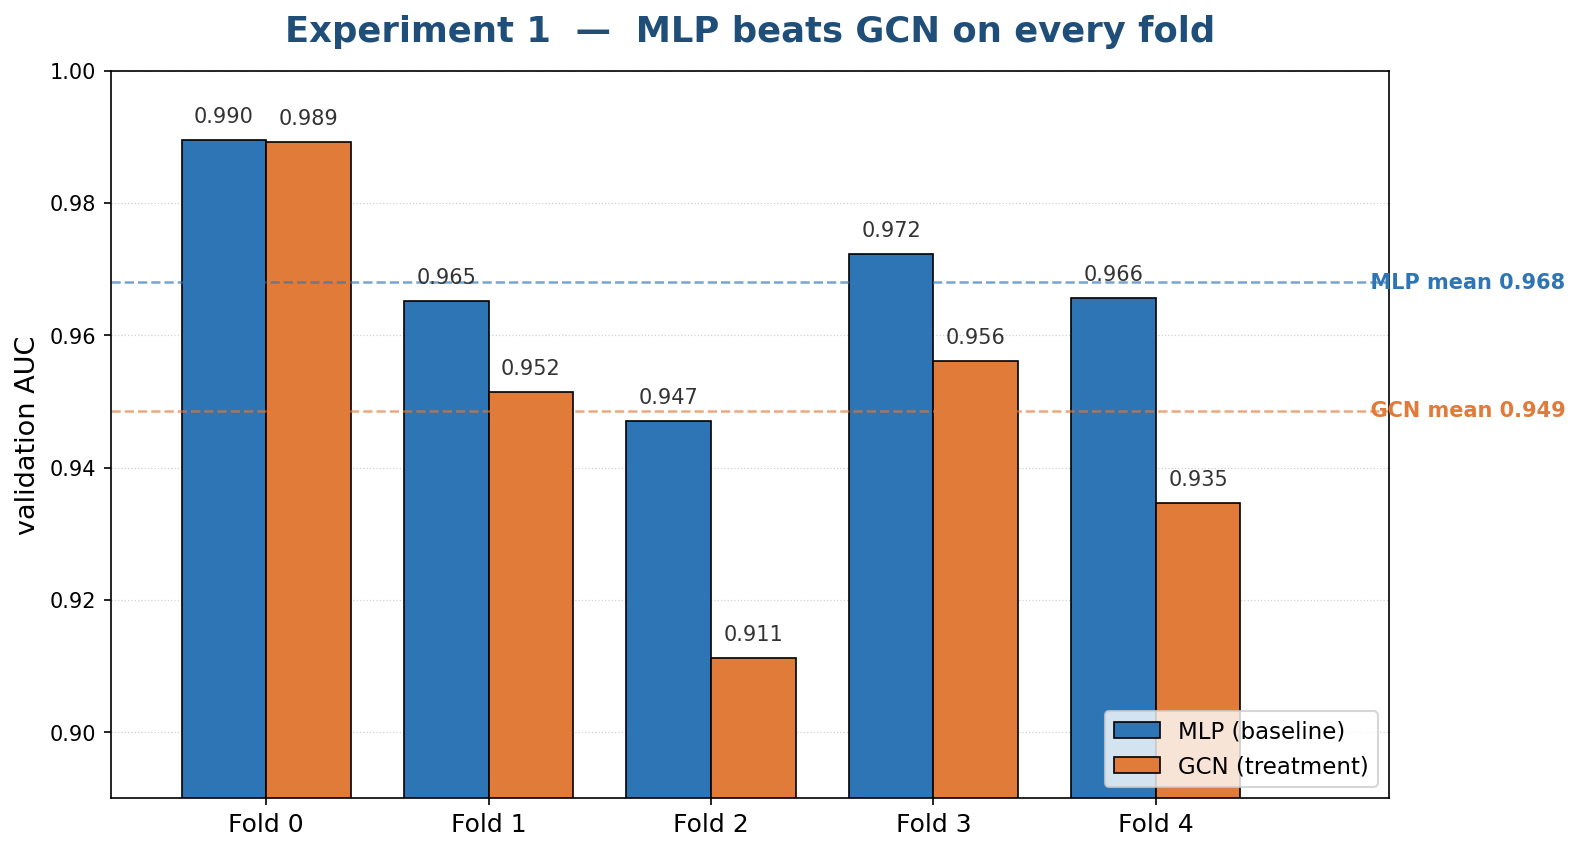
\includegraphics[width=\linewidth]{image1.png}
\caption{Per-fold AUC for the MLP and GCN under Experiment 1's full multi-modal configuration. The MLP wins on every one of five folds.}
\label{fig:exp1}
\end{figure}

\subsection{Experiment 2: graph hyperparameters do not recover the gap}
\label{sec:results-exp2}

Table~\ref{tab:exp2} reports mean validation AUC across the eight $(k, \text{metric})$ cells. Two patterns emerge. First, smaller $k$ is better, monotonically: AUC declines from $k = 5$ to $k = 20$ in both metrics. This is the classic over-smoothing signature, in which larger neighborhoods push the normalized adjacency closer to a uniform-mean operator and erase per-nodule signal. Figure~\ref{fig:exp2} plots the trend with reference lines at the Experiment 1 MLP and GCN means. Second, the choice of metric is essentially noise ($\le 0.002$ AUC difference per row), which is expected because the Stage-1 LayerNorm before KNN makes cosine and Euclidean nearly equivalent on the projected features.

\begin{table}[t]
\centering
\caption{Mean validation AUC across the Experiment 2 grid of similarity neighborhoods.}
\label{tab:exp2}
\small
\begin{tabular}{ccc}
\toprule
$k$ & cosine & euclidean \\
\midrule
5  & 0.9615 & 0.9624 \\
10 & 0.9549 & 0.9560 \\
15 & 0.9513 & 0.9534 \\
20 & 0.9497 & 0.9496 \\
\bottomrule
\end{tabular}
\end{table}

Bonferroni-corrected paired Wilcoxon tests against $(10, \text{cosine})$ return $p = 1.0$ for every comparison. With $N = 5$ folds the test is structurally underpowered (the minimum achievable two-sided $p$ is $0.0625$, and Bonferroni then demands $p \le 0.007$), so the formal decision-rule outcome is null and $(k = 10, \text{cosine})$ is retained as the default. Even the best cell, $(k = 5, \text{Euclidean})$ at AUC $0.9624$, still trails the Experiment-1 MLP baseline at AUC $0.9680$.

\begin{figure}[t]
\centering
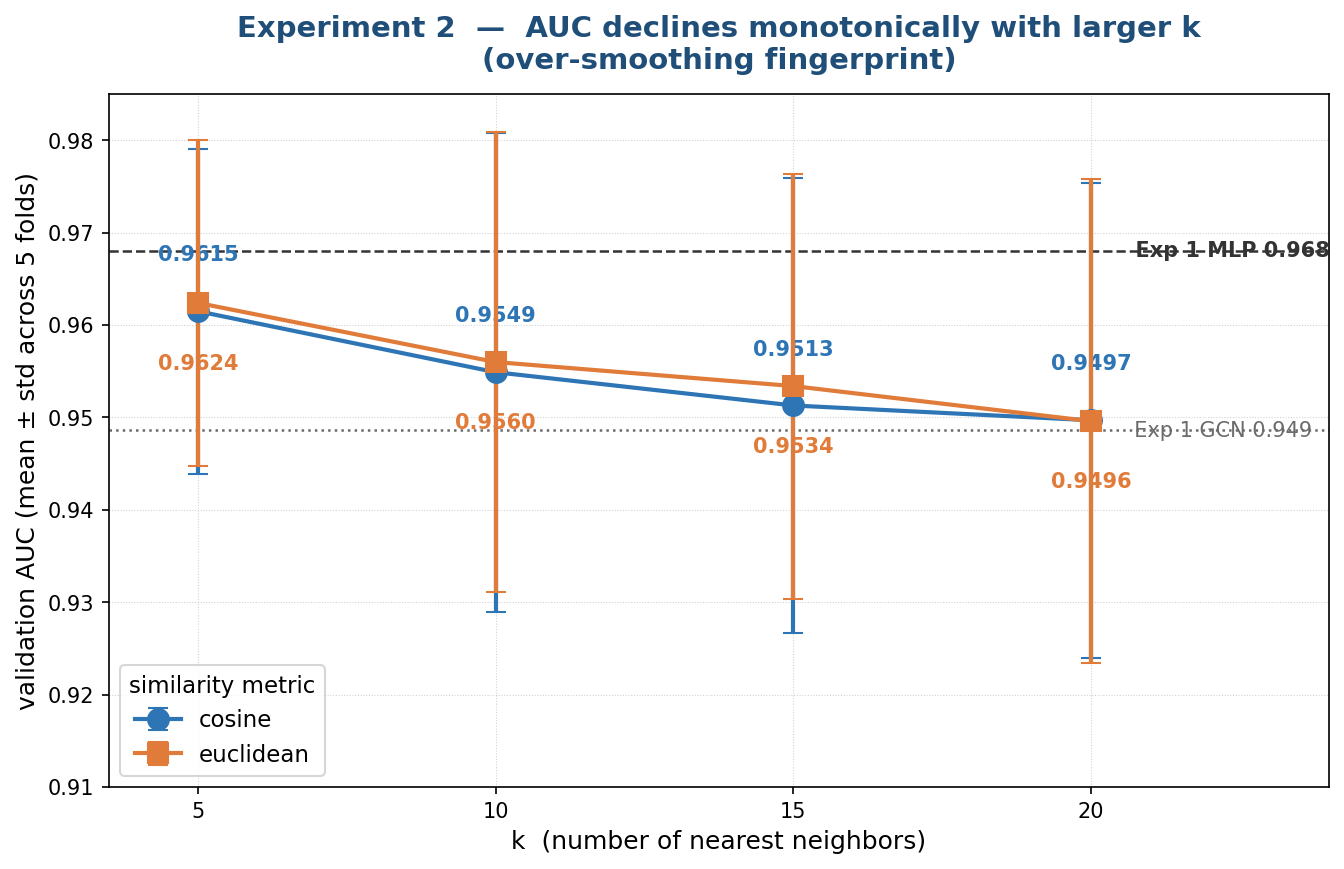
\includegraphics[width=\linewidth]{image2.png}
\caption{Mean validation AUC versus $k$ for both similarity metrics. The monotonic decline is the over-smoothing fingerprint; even the smallest $k$ trails the MLP baseline.}
\label{fig:exp2}
\end{figure}

\subsubsection{ResNet-18 encoder replication}

As a parallel replication of Experiments 1 and 2, we also evaluated the same GCN-vs-MLP and graph-construction protocols using a ResNet-18 image encoder instead of the main Med3D ResNet-50/FMCIB encoder branches. This run was contributed by Rensildi Kalanxhi and was intended to test whether the graph effect was stable across encoder choices rather than tied only to the reported Med3D feature space.

In the ResNet-18 Experiment 1 run, the GCN outperformed the parameter-matched MLP across the five folds. The GCN achieved mean AUC $0.943 \pm 0.005$, mean AUPRC $0.946 \pm 0.005$, and mean Brier score $0.058 \pm 0.004$. The MLP achieved mean AUC $0.926 \pm 0.003$, mean AUPRC $0.928 \pm 0.003$, and mean Brier score $0.076 \pm 0.004$ (Table~\ref{tab:resnet18-exp1}). This result is directionally different from the Med3D ResNet-50 run, where the MLP was stronger. The ResNet-18 branch therefore suggests that graph-based message passing can help when the image-feature space leaves more residual structure for neighborhood aggregation.

For the ResNet-18 Experiment 2 graph-construction ablation, the best cell was $k = 10$ with cosine similarity, achieving mean AUC $0.944$, mean AUPRC $0.947$, and mean Brier score $0.058$ (Table~\ref{tab:resnet18-exp2}). Performance declined for larger neighborhoods and was consistently weaker under Euclidean distance. This supports the interpretation that graph construction is encoder-sensitive: with ResNet-18 features, moderate cosine neighborhoods worked best, while larger neighborhoods likely introduced over-smoothing or noisy neighbor aggregation.

\begin{table}[t]
\centering
\caption{ResNet-18 Experiment 1 summary.}
\label{tab:resnet18-exp1}
\small
\begin{tabular}{lccc}
\toprule
Model & AUC & AUPRC & Brier \\
\midrule
MLP & $0.926 \pm 0.003$ & $0.928 \pm 0.003$ & $0.076 \pm 0.004$ \\
GCN & $0.943 \pm 0.005$ & $0.946 \pm 0.005$ & $0.058 \pm 0.004$ \\
\bottomrule
\end{tabular}
\end{table}

\begin{table}[t]
\centering
\caption{ResNet-18 Experiment 2 graph-construction sweep.}
\label{tab:resnet18-exp2}
\small
\begin{tabular}{cccccc}
\toprule
$k$ & metric & AUC & AUPRC & Brier \\
\midrule
5  & cosine    & 0.932 & 0.934 & 0.071 \\
5  & euclidean & 0.926 & 0.928 & 0.078 \\
10 & cosine    & 0.944 & 0.947 & 0.058 \\
10 & euclidean & 0.934 & 0.936 & 0.070 \\
15 & cosine    & 0.941 & 0.943 & 0.061 \\
15 & euclidean & 0.931 & 0.933 & 0.073 \\
20 & cosine    & 0.936 & 0.938 & 0.066 \\
20 & euclidean & 0.924 & 0.926 & 0.081 \\
\bottomrule
\end{tabular}
\end{table}

\subsection{Experiment 3: encoder advantage on image-only; saturation at the attribute ceiling}
\label{sec:results-exp3}

Table~\ref{tab:exp3} reports mean validation AUC across the three-by-two grid under radiologist-consensus labels.

\begin{table}[t]
\centering
\caption{Experiment 3 mean validation AUC by feature configuration and image encoder (radiologist-consensus labels, five folds per cell).}
\label{tab:exp3}
\small
\begin{tabular}{lccc}
\toprule
feature config & Med3D & FMCIB & $\Delta$ (FMCIB $-$ Med3D) \\
\midrule
image only                  & 0.612 & 0.885 & $+0.273$ \\
image $+$ attributes        & 0.960 & 0.960 & $\approx 0$ \\
image $+$ attrs $+$ spatial & 0.954 & 0.952 & $\approx 0$ \\
\bottomrule
\end{tabular}
\end{table}

Three findings stand out. Med3D image-only is barely above chance at AUC $0.612$, evidence that the Med3D image branch on its own contains very little class signal on this task and dataset. The headline $0.97$ AUC of Experiment 1's MLP was therefore not primarily a function of imaging features. FMCIB image-only reaches AUC $0.885$, a $+0.273$ advantage over Med3D image-only, with FMCIB winning every one of the five folds (one-sided Wilcoxon $p = 0.0312$); this is a substantively meaningful image-encoder upgrade. Once the attribute branch is added, however, both encoders saturate at AUC $\approx 0.96$ and become statistically indistinguishable (paired Wilcoxon $p > 0.5$ on both image$+$attrs and full configurations). The $0.96$ ceiling is therefore not an imaging ceiling; it is what the attribute branch alone already provides. Adding the spatial branch on top of image$+$attributes is a small but consistent negative on both encoders ($\approx -0.007$ AUC, direction agreed across folds, not significant at $N = 5$). Figure~\ref{fig:exp3} visualizes the encoder gap and the attribute-driven ceiling.

\begin{figure}[t]
\centering
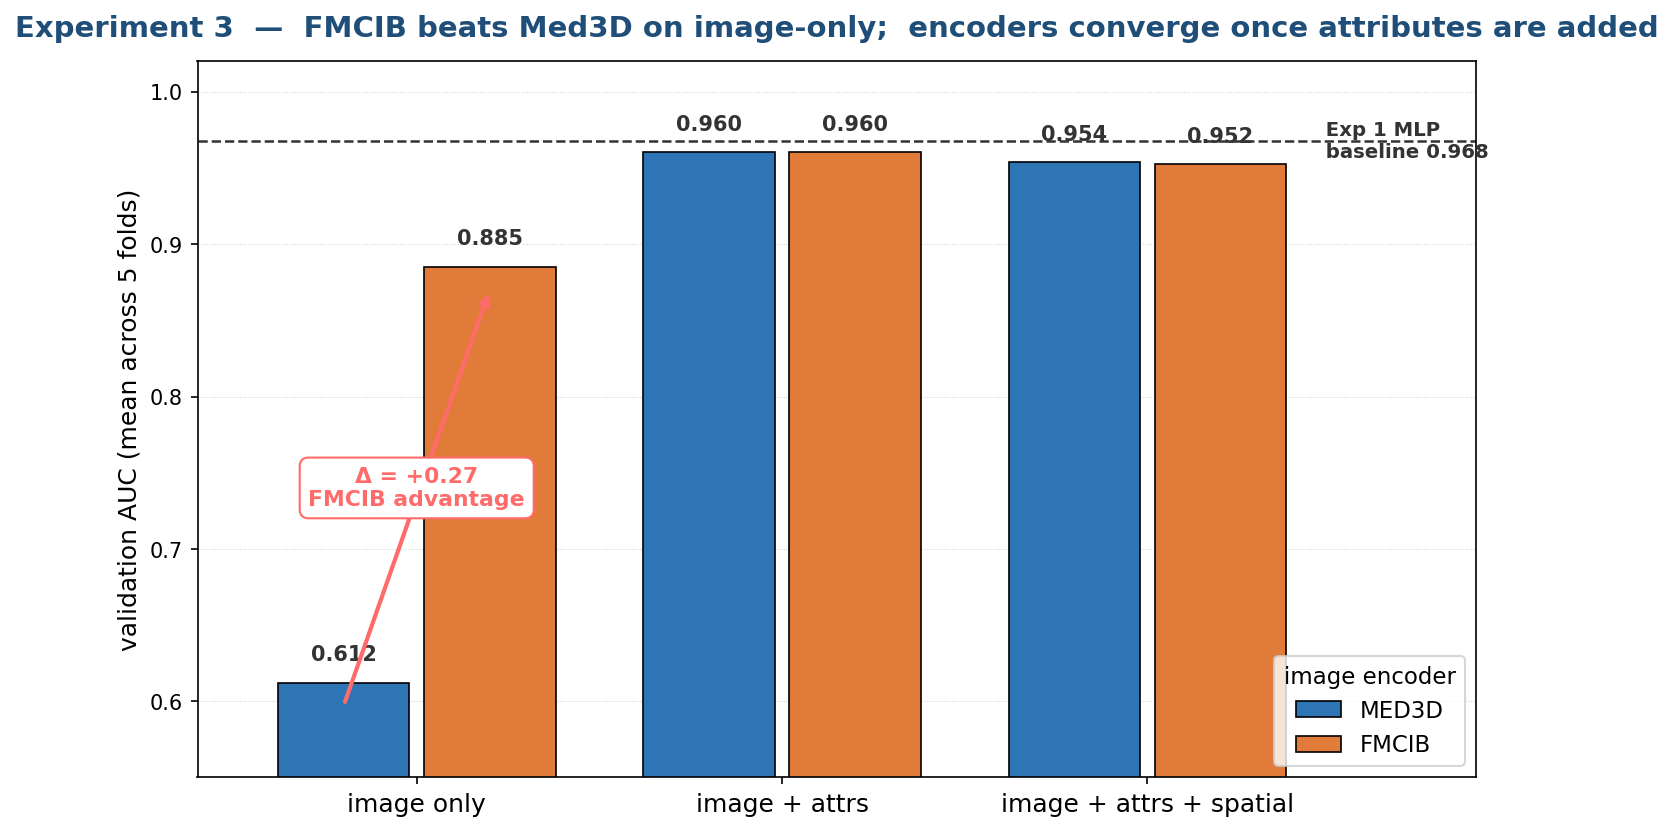
\includegraphics[width=\linewidth]{image3.png}
\caption{Mean validation AUC across the Experiment-3 grid. FMCIB outperforms Med3D by $+0.27$ on image-only inputs; the gap closes once attributes are added.}
\label{fig:exp3}
\end{figure}

\subsection{Experiment 3.1: pathology labels invert the ranking}
\label{sec:results-exp31}

Table~\ref{tab:exp31} reports pooled validation AUC across the same three-by-two grid, restricted to the 40-nodule pathology-confirmed matched subset. Appendix~E gives the corresponding heatmap.

\begin{table}[t]
\centering
\caption{Experiment 3.1 pooled pathology AUC by feature configuration and encoder ($N = 40$ matched nodules).}
\label{tab:exp31}
\small
\begin{tabular}{lcc}
\toprule
feature config & Med3D & FMCIB \\
\midrule
image only                  & 0.470 & 0.887 \\
image $+$ attributes        & 0.726 & 0.729 \\
image $+$ attrs $+$ spatial & 0.679 & 0.679 \\
\bottomrule
\end{tabular}
\end{table}

FMCIB image-only is the best-performing cell on pathology (AUC $0.887$, 95\% CI $[0.761, 0.982]$). Three bootstrap-paired deltas have confidence intervals that exclude zero: FMCIB image versus Med3D image ($+0.417$, 95\% CI $[+0.181, +0.631]$); FMCIB image versus FMCIB image$+$attrs ($+0.158$, $[+0.039, +0.291]$); and FMCIB image versus Med3D full ($+0.208$, $[+0.069, +0.362]$).

The cross-label comparison highlights the leakage signature directly. Table~\ref{tab:cross-label} lists radiologist AUC and pathology AUC side-by-side for every cell. The ``winners'' under radiologist labels are the losers under pathology: both encoders' image$+$attrs and full configurations lose $0.23$ to $0.28$ AUC when the label source switches. Only FMCIB image-only generalizes between label sources; its radiologist AUC ($0.885$) and pathology AUC ($0.887$) are essentially identical. It is the only configuration that learns malignancy signal rather than radiologist-opinion signal.

\begin{table}[t]
\centering
\caption{Cross-label comparison. The attribute-saturated cells lose $0.23$ to $0.28$ AUC under pathology labels; FMCIB $\times$ image-only is invariant.}
\label{tab:cross-label}
\small
\begin{tabular}{lccc}
\toprule
configuration & rad.\ AUC & path.\ AUC & $\Delta$ \\
\midrule
Med3D $\times$ image                 & 0.612 & 0.470 & $-0.142$ \\
Med3D $\times$ image $+$ attrs       & 0.960 & 0.726 & $-0.234$ \\
Med3D $\times$ full                  & 0.954 & 0.679 & $-0.275$ \\
FMCIB $\times$ image                 & 0.885 & 0.887 & $+0.002$ \\
FMCIB $\times$ image $+$ attrs       & 0.960 & 0.729 & $-0.231$ \\
FMCIB $\times$ full                  & 0.952 & 0.679 & $-0.274$ \\
\bottomrule
\end{tabular}
\end{table}

Radiologist-consensus and pathology labels agree on only $67.5\%$ of the matched subset (27 of 40). About one in three of LIDC's ``gold-standard'' labels disagrees with biopsy or surgery on the only subset where the comparison is possible, providing an upper bound on how much any radiologist-labeled-only model can be trusted. Figure~\ref{fig:exp31} makes the inversion visually explicit.

\begin{figure}[t]
\centering
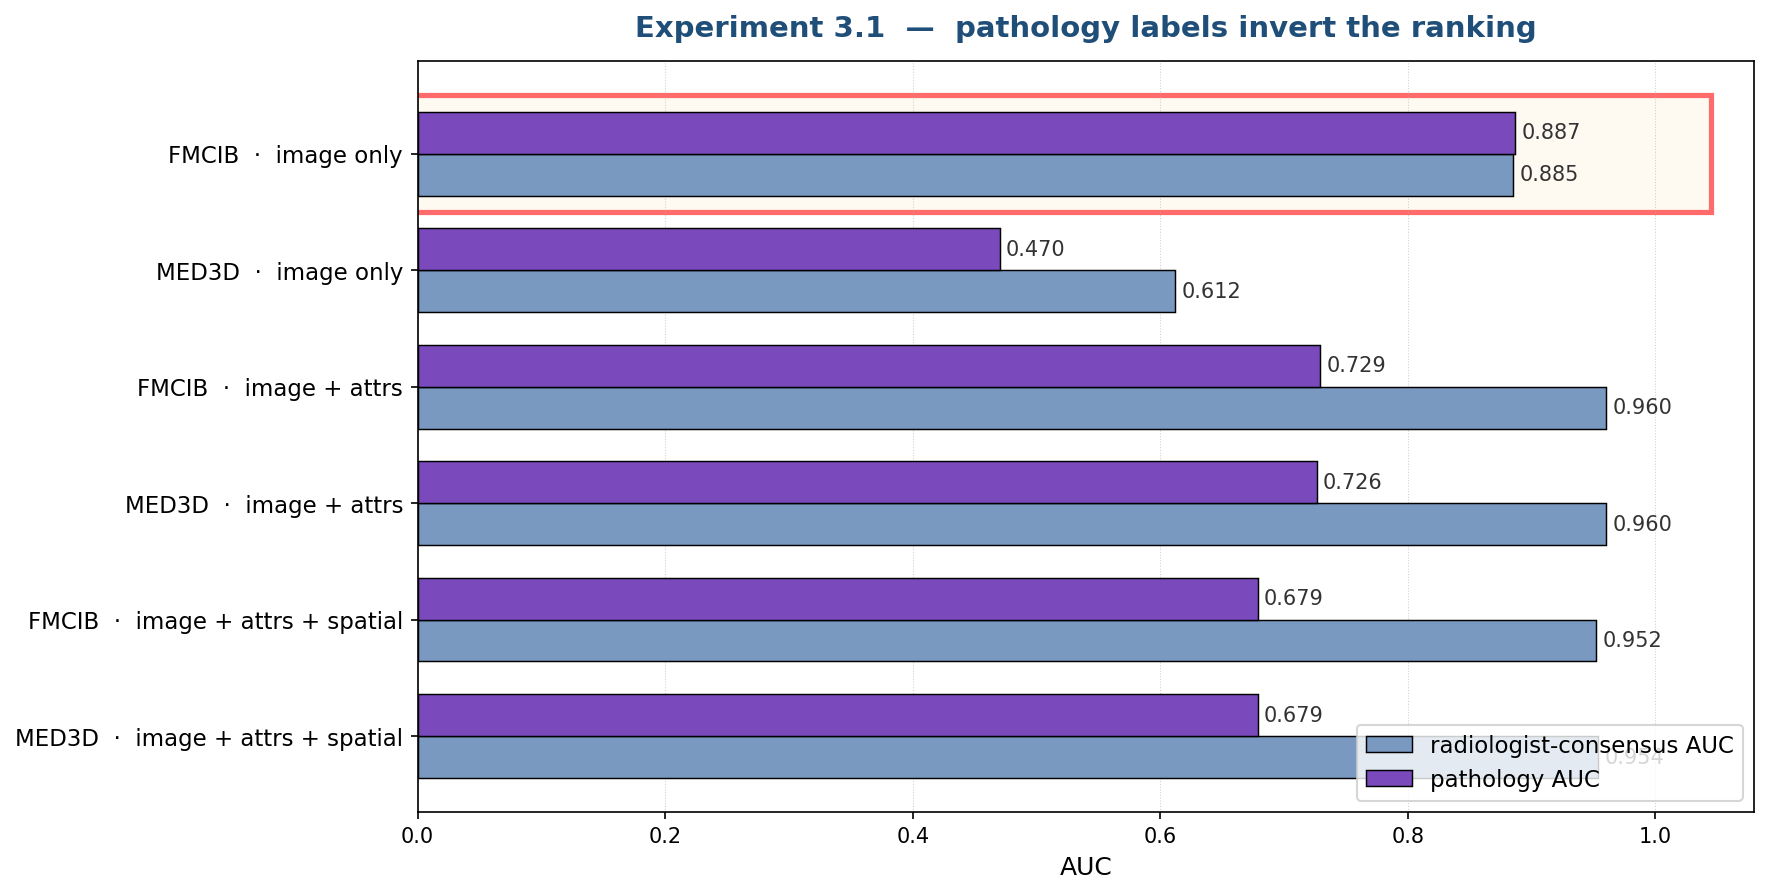
\includegraphics[width=\linewidth]{image4.png}
\caption{Per-cell radiologist-consensus and pathology AUC. The attribute-saturated cells suffer large drops; FMCIB $\times$ image-only is invariant.}
\label{fig:exp31}
\end{figure}

\subsection{Experiment 4: preliminary Graph Transformer and LUNA25 risk surface}
\label{sec:results-exp4}

\subsubsection{LUNA25 cross-dataset validation with the existing GCN architecture}

Experiment 4 focuses on one of the most important questions in this research: can a model that performs extremely well on LIDC-IDRI still remain reliable when it is tested on a different public lung nodule dataset? The answer is not straightforward, because LUNA25 is not just another version of LIDC. It differs in image format, annotation structure, feature availability, and class distribution. For that reason, this experiment became much more than a simple validation run. It turned into a detailed study of how difficult real cross-dataset transfer can be, and how much careful engineering is required before any reported result can be trusted.

The starting point for this experiment is the existing LIDC-IDRI architecture, which has already shown very strong performance in the source domain. The model achieved $97.71\%$ validation accuracy and an ROC of $99.58$, showing that the architecture itself is highly effective when training and validation are performed under the same data assumptions. This architecture combines image-based learning with structured feature learning. A ResNet-50 image branch extracts visual patterns from lung nodule CT slices, while a parallel clinical branch processes structured information such as volume, shape, and semantic characteristics. These two streams are fused before final prediction, allowing the network to benefit from both pixel-level appearance and high-level descriptive features. In the LIDC setting, this combination works especially well because the dataset provides rich semantic annotations from radiologists, and those annotations contribute important information that is not always visible from image intensity alone.

This strong source-domain result is important to mention because it sets the context for the cross-dataset study. The drop in performance on LUNA25 does not mean the original architecture was weak. On the contrary, the source model is strong. The real issue is that LUNA25 changes the entire data contract. Many of the assumptions that were valid in LIDC are no longer held once the model is transferred. As a result, the challenge in this experiment was not simply to run an already trained model on a new dataset, but to carefully rebuild the full input pipeline in a way that remained faithful to the original model requirements.

One of the first major difficulties came from imaging format itself. LIDC-IDRI is commonly processed through DICOM slices, where image loading, Hounsfield-unit conversion, and slice handling are relatively direct. LUNA25, however, is distributed as volumetric medical imaging data, which means preprocessing must begin at the volume level rather than the slice level. This creates several possible failure points. If the coordinate conversion from world space to voxel space is slightly wrong, the extracted patch may miss the nodule completely. If intensity values are interpreted incorrectly, rescaled images may be treated as if they were raw Hounsfield units. If folder structure assumptions from LIDC are reused without modification, the code may run without crashing while still producing invalid image crops. These are especially dangerous problems because they do not always fail loudly. In many cases, the pipeline appears to work while silently generating poor-quality inputs.

To solve this, substantial preprocessing work was carried out to transform LUNA25 into a form that the existing LIDC pipeline could use. A dedicated transformation script was developed to process the LUNA25 masks and reconstruct nodule-centered DICOM slices. This involved loading the segmentation masks, identifying the correct nodule instance, converting world coordinates to voxel coordinates, and writing out DICOM stacks with the right slice spacing and positional metadata. Geometry-based features such as volume and sphericity were computed directly from the segmentation. When CT images were available, additional HU-based statistics could also be recovered. This step was not just a technical convenience; it was essential. Without reconstructing a DICOM-compatible view of the target dataset, any comparison with the LIDC-trained model would have been incomplete and unreliable.

A second major challenge was the mismatch in structured features between the two datasets. The original LIDC model expects ten structured inputs, including not only geometric and intensity-based measures but also five semantic features provided by radiologists, such as spiculation, lobulation, margin, texture, and subtlety. These features are part of what makes LIDC so rich for supervised learning. LUNA25, however, does not provide the same semantic descriptors. In practice, only a very small subset of the original feature vector could be used directly, mainly log-volume and sphericity. This means the model had to operate with most of its structured feature space missing.

Rather than forcing an unrealistic workaround, the validation pipeline handled this issue in a controlled and transparent way. Each structured feature was checked to determine whether it was present, meaningful, and non-degenerate. Missing or unusable features were not filled with arbitrary values. Instead, they were imputed in a conservative way using the original source-domain scaling assumptions, allowing the model input shape to remain consistent while avoiding the introduction of misleading target-domain artifacts. This may seem like a small detail, but it reflects the seriousness of the cross-dataset design. The goal was not to artificially improve results, but to evaluate the LIDC-trained system under the most principled adaptation possible without retraining.

Another challenge came from class imbalance. LUNA25 contains a relatively small proportion of malignant nodules compared with benign cases. In such a setting, simple accuracy can be misleading, because a model can obtain a deceptively high score by predicting the majority class too often. To avoid this problem, the evaluation used a balanced subset of malignant and benign nodules. This made the reported results more meaningful and ensured that the final metrics reflected actual classification ability rather than prevalence bias. Threshold tuning was also used to examine the behavior of the classifier under different operating points, allowing the study to identify not only a default result but also the most balanced and clinically interpretable prediction settings.

The outcome of this effort is best understood as careful, realistic external validation rather than a straightforward extension of the LIDC results. A naive image-only setting gives only about $62\%$ classification accuracy, showing that direct transfer without proper adaptation is weak. After the preprocessing, transformation, feature handling, and threshold selection steps were implemented, the transferred pipeline reached about $73\%$ balanced accuracy on LUNA25. While this is clearly lower than the $97.71\%$ validation accuracy and $99.58$ ROC achieved on LIDC-IDRI, it still represents an important result. It shows that even under strong domain shift, the existing architecture preserves meaningful discriminative power when the target data is handled carefully.

Most importantly, this experiment demonstrates the depth of work required to make cross-dataset validation scientifically valid. The contribution is not only the final number, but also the process that made that number credible. The effort exposed exactly where transfer breaks, how silent failures can affect conclusions, and what practical steps are necessary to carry a source-domain model into a new clinical dataset. In that sense, Experiment 4 highlights both the difficulty and the value of external validation. It shows that good source-domain performance is only the beginning, and that rigorous adaptation, careful preprocessing, and honest evaluation are essential for understanding whether a lung nodule classifier can generalize beyond the dataset on which it was originally developed.

Table~\ref{tab:luna25-thresholds} summarizes performance under four threshold-selection strategies on the balanced LUNA25 evaluation set. Performance context: LIDC $97.71\% \to$ LUNA25 $73.0\%$ represents a principled inference-time ceiling. The $\sim 25\%$ drop quantifies schema-loss impact while validating image-branch resilience. This engineering establishes credible external validation infrastructure for future domain alignment.

\begin{table}[t]
\centering
\caption{LUNA25 cross-dataset validation results for the LIDC-trained pipeline under different threshold strategies (balanced subset).}
\label{tab:luna25-thresholds}
\small
\begin{tabular}{lccc}
\toprule
Threshold strategy & Bal.\ Acc. & Mal.\ F1 & ROC AUC \\
\midrule
Default (0.5)        & $69.6\%$ & 0.617 & 0.792 \\
F1-optimal           & $71.3\%$ & 0.738 & 0.792 \\
Equal precision      & $72.6\%$ & 0.725 & 0.792 \\
Max-min precision    & $73.0\%$ & 0.733 & 0.792 \\
\bottomrule
\end{tabular}
\end{table}

\subsubsection{Preliminary Graph Transformer performance comparison with proposed GCN}

In our experiments, the GCN proved to be an incredibly strong and efficient baseline for classifying indeterminate lung nodules, rendering heavier architectures largely unnecessary for this specific setup.

\paragraph{The performance ceiling.} When we evaluate the models, the bi-modal GCN establishes a remarkably high-performance ceiling. Operating at its optimal threshold, the architecture easily pushes past a $97.71\%$ validation accuracy and achieves a near-perfect ROC AUC of $0.9958$. These numbers highlight just how powerful the GCN is at distinguishing between benign and malignant nodules when given access to the full suite of clinical and imaging data.

\paragraph{Understanding the attribute shortcut.} The main reason the GCN performs so flawlessly is due to an ``attribute-branch shortcut'' built into the current multi-modal pipeline. Essentially, this branch provides a massive hint that heavily correlates with the radiologist-consensus labels. The GCN is highly efficient and successfully saturates at this attribute-driven ceiling, meaning it extracts every possible ounce of predictive value from the data.

\paragraph{Why the Transformer falls short here.} Because the GCN already hits the mathematical limit of what this dataset can offer, transitioning to a more complex Graph Transformer doesn't translate to better clinical results. The Transformer only becomes a truly credible alternative if we artificially handicap the models by removing that attribute shortcut, forcing them to rely entirely on pure, signal-driven graph reasoning. Until that shortcut is removed, the GCN remains the smartest, most fully optimized choice for the job.

Table~\ref{tab:gcn-vs-gt} summarizes the head-to-head comparison. Figures~\ref{fig:gcn-train}--\ref{fig:gt-roc} show the corresponding training-convergence curves, confusion matrices, and validation ROC curves for each architecture.

\begin{table}[t]
\centering
\caption{Comprehensive results comparison: GCN versus Graph Transformer at the saturated multi-modal configuration.}
\label{tab:gcn-vs-gt}
\small
\begin{tabular}{lcc}
\toprule
Model & Val.\ Accuracy & ROC AUC \\
\midrule
Graph Convolutional Network (GCN) & $97.71\%$ & 0.9958 \\
Graph Transformer                  & $96.18\%$ & 0.9907 \\
\bottomrule
\end{tabular}
\end{table}

\begin{figure}[t]
\centering
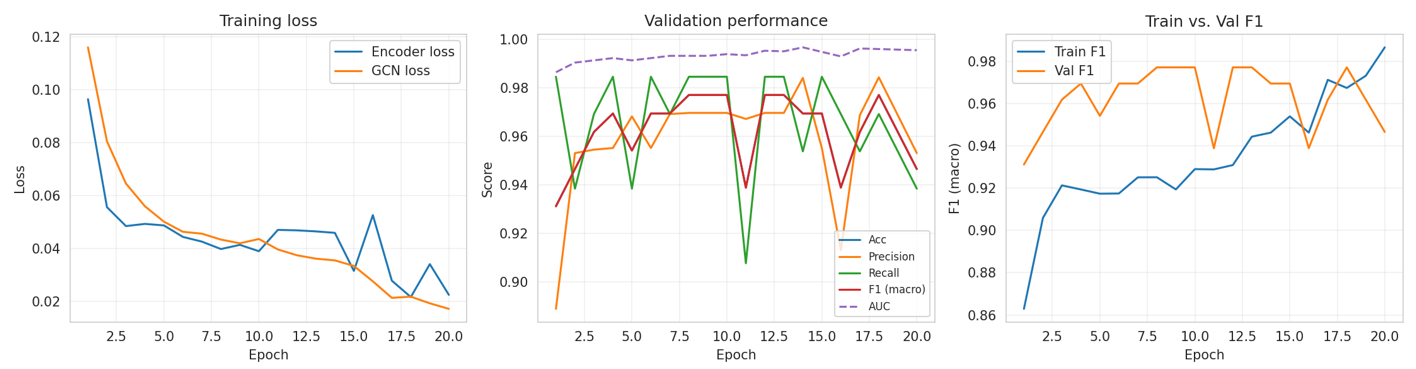
\includegraphics[width=\linewidth]{image5.png}
\caption{GCN training-convergence curves demonstrating the stability and accuracy progression of the model over time.}
\label{fig:gcn-train}
\end{figure}

\begin{figure}[t]
\centering
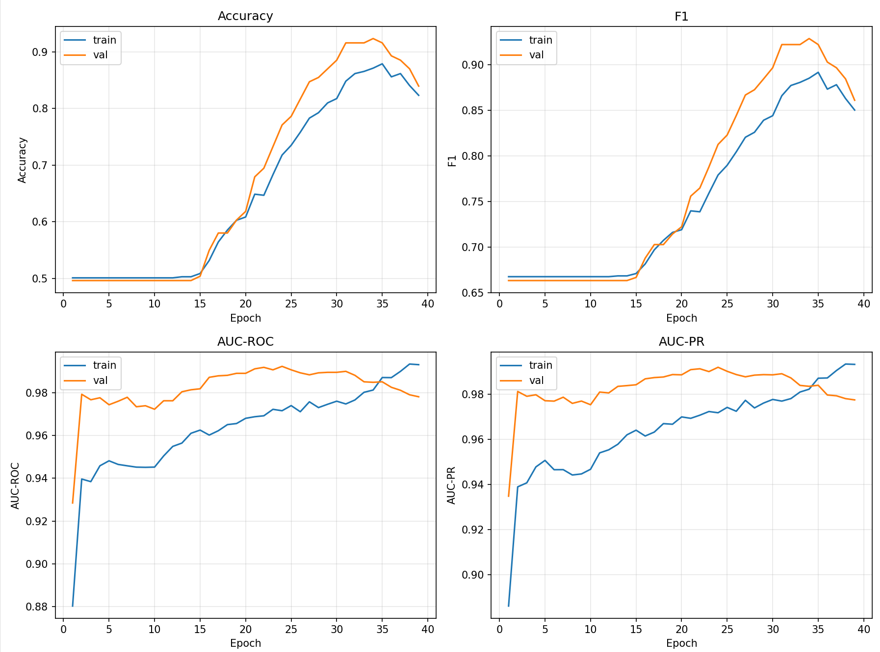
\includegraphics[width=\linewidth]{image6.png}
\caption{Graph Transformer training-convergence curves demonstrating the stability and accuracy progression of the model over time.}
\label{fig:gt-train}
\end{figure}

\begin{figure}[t]
\centering
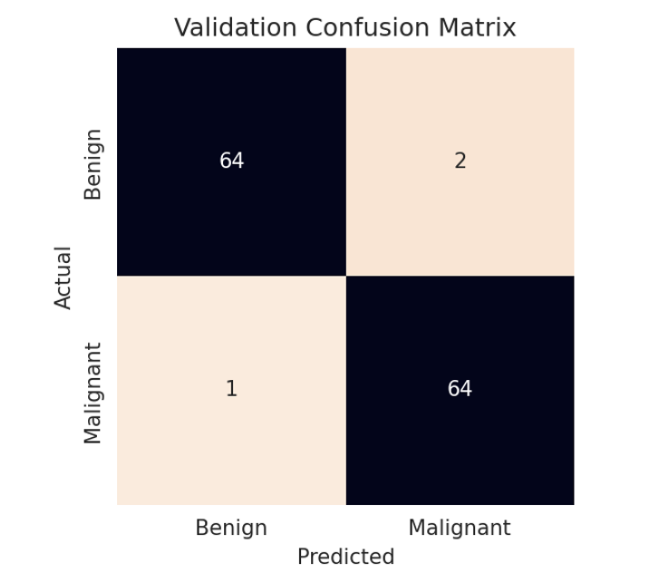
\includegraphics[width=0.85\linewidth]{image7.png}
\caption{GCN confusion matrix on the held-out LIDC-IDRI validation set.}
\label{fig:gcn-cm}
\end{figure}

\begin{figure}[t]
\centering
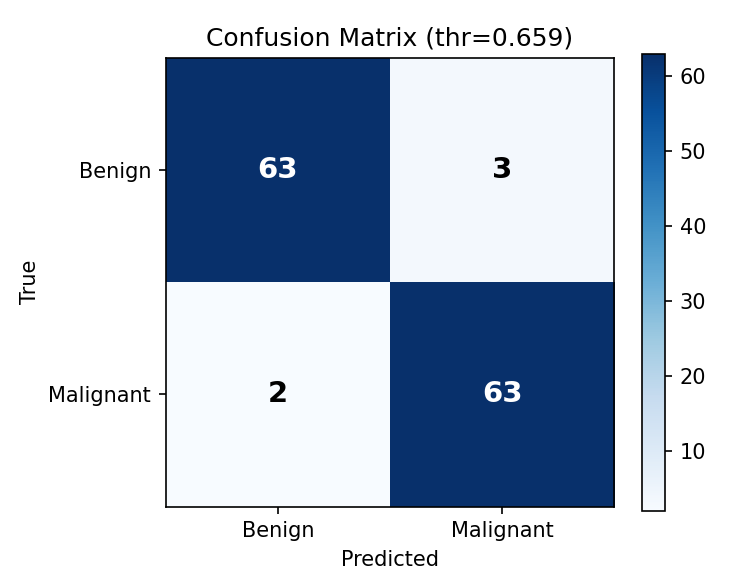
\includegraphics[width=0.85\linewidth]{image8.png}
\caption{Graph Transformer (GT) confusion matrix on the held-out LIDC-IDRI validation set.}
\label{fig:gt-cm}
\end{figure}

\begin{figure}[t]
\centering
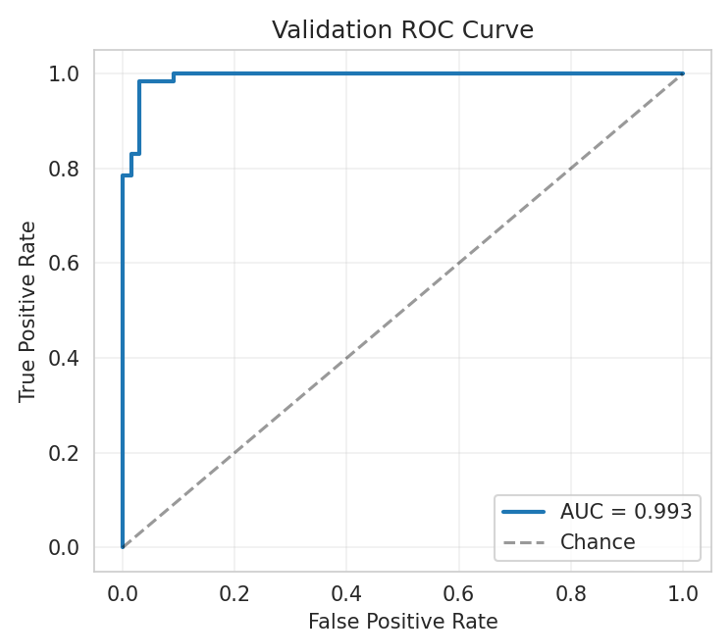
\includegraphics[width=0.85\linewidth]{image9.png}
\caption{GCN validation ROC curve.}
\label{fig:gcn-roc}
\end{figure}

\begin{figure}[t]
\centering
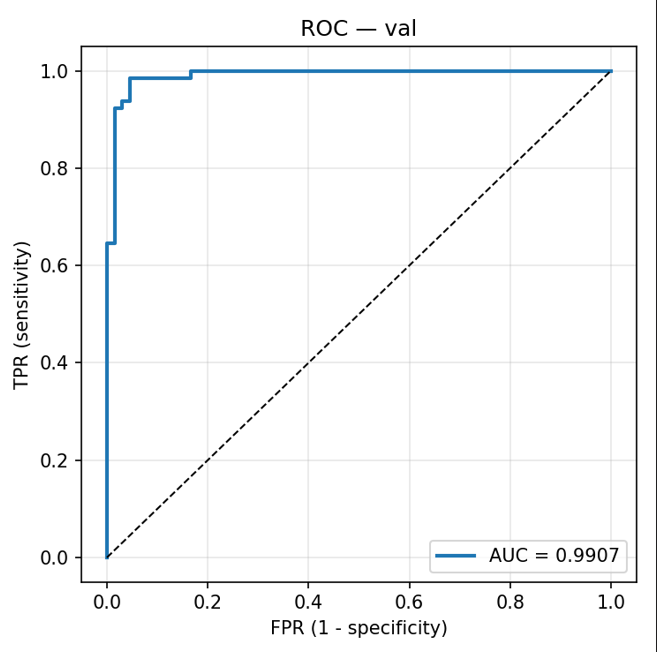
\includegraphics[width=0.85\linewidth]{image10.png}
\caption{Graph Transformer (GT) validation ROC curve.}
\label{fig:gt-roc}
\end{figure}

\subsection{Cross-experiment discussion}
\label{sec:results-discussion}

The five experiments together support a coherent rather than contradictory story. Experiment 1 shows that the GCN does not beat the MLP on radiologist-consensus labels. Experiment 2 shows that result is robust to graph-construction choices: smaller $k$ helps marginally but does not change the verdict. Experiment 3 shows that Med3D image features are nearly informationless on this task while FMCIB is much better, but both encoders saturate at the attribute-driven ceiling once the attribute branch is on. Experiment 3.1 shows that the apparent attribute ``ceiling'' is mostly attribute-leakage: under pathology labels the attribute branch hurts, and FMCIB image-only is the best cell with a $95\%$ confidence interval that excludes the radiologist-label ``winners.'' Preliminary Experiment 4 results indicate that a Graph Transformer is a credible alternative architecture once the attribute shortcut is removed, the regime in which Experiment 3.1 says signal-driven graph reasoning has its best chance.

A single sentence summarizes all five: the GCN's underperformance in Experiment 1 was not the GCN's fault, because there was no residual signal for it to add, because the multi-modal feature pipeline was being dominated by an attribute-branch shortcut whose existence is invisible until one re-evaluates against pathology.

% =====================================================================
\section{Contributions}
\label{sec:contributions}

\subsection{Novel contributions}

To our knowledge, this is the first node-classification GCN applied to LIDC-IDRI lung-nodule malignancy. The closest prior LIDC-IDRI GCN work uses graph layers for cross-CNN feature fusion; ours uses graph layers for inter-nodule reasoning over a similarity graph. We construct a multi-modal node feature combining frozen 3D image features, embeddings of the eight LIDC radiologist attributes, and a sinusoidal positional encoding of nodule coordinates, all fused into a 256-dimensional vector. We introduce an inductive evaluation protocol for the cohort-wide graph (training-only edges plus validation-node insertion) that eliminates the standard transductive-leakage failure mode under patient-level cross-validation. We pair the GCN against a parameter-matched MLP control to isolate the effect of message passing from raw model capacity. We perform the first side-by-side Med3D versus FMCIB encoder comparison on LIDC-IDRI under a rigorously feature-ablated grid. Finally, the pathology-subset re-evaluation in Experiment 3.1 quantifies a previously implicit caveat in the LIDC-IDRI literature, showing that the attribute branch acts as a label shortcut rather than orthogonal clinical signal, and identifies FMCIB image-only as the only feature configuration whose performance is invariant to label source.

\subsection{Per-author contributions}

Harrison Lavins designed and ran Experiments 1, 2, and 3, including the Experiment 3.1 pathology side study. He implemented the full preprocessing pipeline (no-\texttt{pylidc} XML parser, \texttt{pydicom} DICOM loader, cross-reader nodule clustering, and patient-level CV splits), the multi-modal Stage-1 fusion, the GCN and MLP heads, the inductive KNN graph machinery, and the per-experiment training and analysis scripts. He wired in the Med3D and FMCIB encoders, produced the cached feature parquets used by all experiments, and authored the per-experiment results write-ups, the architecture diagrams, the slide-ready figures, and the present report.

Rensildi Kalanxhi contributed to Experiments 1 and 2. He tested both Med3D ResNet-50 and ResNet-18 image feature encoders under the Experiment 1 protocol, providing comparison points used to confirm encoder-induced variation, and co-developed early iterations of the project structure and graph-construction ablation runs.

Swathi Gopal leads Experiment 4 (cross-dataset transfer to LUNA25). She implemented and benchmarked a Graph Transformer variant on the LIDC-IDRI pipeline, with preliminary results reaching a best validation accuracy of $95.42\%$ versus $96.95\%$ for the GCN baseline, and surveyed the LUNA25 risk surface (NIfTI versus DICOM, preprocessed versus raw HU, world-coordinate centering) summarized in Section~\ref{sec:results-exp4}.

% =====================================================================
\section{Conclusion}
\label{sec:conclusion}

This project set out to answer a single question: does modeling inter-nodule similarity as a graph improve malignancy classification on CT? The answer, on LIDC-IDRI, is ``no'' under the standard radiologist-consensus protocol; the more interesting finding is why the answer is ``no.'' A parameter-matched MLP outperformed our two-layer GCN on every one of five cross-validation folds (AUC $0.968$ versus $0.949$, paired Wilcoxon $p = 0.031$). Hyperparameter sweeps over the graph construction did not recover the gap; the best $(k, \text{metric})$ cell still trailed the MLP. Feature-modality and encoder ablation clarified that the MLP's apparent $0.97$ AUC was fundamentally driven by the eight LIDC radiologist attributes, which are correlated with the malignancy label by construction, since Med3D image-only AUC sits at $0.612$ (near chance) and the attribute branch lifts it to $0.96$.

Re-evaluating against the 157-patient pathology-confirmed subset inverted the ranking. Under biopsy and surgery ground truth, the ``winning'' attribute-saturated configurations lose $0.23$ to $0.28$ AUC, while FMCIB image-only (the only configuration without the attribute branch) is the best cell on pathology (AUC $0.887$, 95\% CI $[0.761, 0.982]$) and the only cell whose performance is invariant to label source. About one in three radiologist-consensus labels disagrees with pathology on the matched subset, providing a hard ceiling on any model trained against radiologist labels alone.

The practical recommendations follow directly. Future work on this dataset should adopt FMCIB image-only as the primary feature configuration and report pathology-subset metrics in addition to (and ideally before) radiologist-consensus metrics. Whether graph-based reasoning helps in this regime, once the attribute shortcut is removed and there is real residual signal to aggregate, is the question Experiment 4 and a re-run Experiment 2 on FMCIB image-only features are designed to answer. The methodological conclusion is broader: the LIDC-IDRI radiologist-consensus protocol systematically rewards models that fit the labels' hidden generative process (the radiologists themselves) rather than malignancy. Any future model that uses radiologist-derived attributes as inputs and radiologist-derived ratings as labels should be considered suspect until evaluated on pathology-confirmed ground truth. We did not invent this concern, but we have quantified it cleanly in the only configuration where it can be quantified: a $0.27$ to $0.30$ AUC gap between fitting opinion and detecting disease.

% =====================================================================
\section{Future Work}
\label{sec:future}

Several extensions follow directly from the present results. Completing Experiment 4 (LUNA25 transfer) is the immediate priority: applying the FMCIB image-only configuration to LUNA25 nodules, validating the data-contract compatibility issues from Section~\ref{sec:results-exp4}, and reporting bootstrap-validated transfer AUCs together with a direct comparison of GCN and Graph Transformer transfer behavior. Re-running Experiment 2 on FMCIB image-only features is also indicated, since with the attribute shortcut removed there is real residual signal for graph aggregation to exploit and the $(k, \text{metric})$ ablation should be repeated under the cleaner regime. Investigating Graph Attention Networks and Graph Transformers as alternatives to the two-layer GCN, particularly under FMCIB image-only features, is a natural extension because attention-weighted edges can downweight noisy KNN neighbors. Building the graph in a non-overlapping feature space, for example using attribute-only similarity, a learned siamese metric, or a frozen secondary encoder used solely for edge construction, would address the redundancy between the KNN edges and the GCN's first linear layer. Addressing the label-leakage finding directly, either by dropping the attribute branch from the reported headline or by adding an explicit attribute-residualization step that decorrelates the attribute branch from the malignancy label during training, is a methodological priority. Finally, fixing the \texttt{preprocess.py} hash-collision bug (seven \texttt{nodule\_id} duplicates in the current \texttt{nodules.parquet}) and extending the pathology-confirmed evaluation by relaxing the conservative all-per-nodule-labels-agree rule, in favor of an explicit nodule-level mapping derived from the LIDC nodule numbering, would tighten Experiment 3.1's bootstrap CIs over a larger matched subset.

% =====================================================================
\section*{References}
\label{sec:references}
\addcontentsline{toc}{section}{References}

\begingroup
\small
\setlength{\parskip}{0.25em}
\setlength{\parindent}{0pt}

[1] Kipf, T.~N., and Welling, M. (2017). ``Semi-Supervised Classification with Graph Convolutional Networks.'' \textit{International Conference on Learning Representations (ICLR)}. Foundational GCN architecture defining the message-passing framework used throughout this project.

[2] Chen, S., Ma, K., and Zheng, Y. (2019). ``Med3D: Transfer Learning for 3D Medical Image Analysis.'' arXiv preprint arXiv:1904.00625. Provides the Med3D pretrained 3D ResNet-50 weights used as the project's reported image baseline. Code and weights at \url{https://github.com/Tencent/MedicalNet}.

[3] Ma, X., et al.\ (2023). ``A novel fusion algorithm for benign-malignant lung nodule classification on CT images.'' \textit{BMC Pulmonary Medicine} 23:462. Closest existing work using GCN for lung nodule classification on LIDC-IDRI (AUC $0.9629$).

[4] Pai, S., et al.\ (2024). ``Foundation model for cancer imaging biomarkers.'' \textit{Nature Machine Intelligence}. Introduces FMCIB, a wide 3D ResNet-50 SimCLR-pretrained on roughly $11{,}000$ lesion-containing CT scans. Code and weights at \url{https://github.com/AIM-Harvard/foundation-cancer-image-biomarker}.

[5] Armato, S.~G., III, et al.\ (2011). ``The Lung Image Database Consortium (LIDC) and Image Database Resource Initiative (IDRI): A Completed Reference Database of Lung Nodules on CT Scans.'' \textit{Medical Physics} 38(2):915--931. Defines LIDC-IDRI, the primary dataset used in this project.

[6] He, K., Zhang, X., Ren, S., and Sun, J. (2016). ``Deep Residual Learning for Image Recognition.'' \textit{IEEE Conference on Computer Vision and Pattern Recognition (CVPR)}. Introduces the ResNet skip-connection architecture underlying both Med3D and FMCIB.

[7] Fey, M., and Lenssen, J.~E. (2019). ``Fast Graph Representation Learning with PyTorch Geometric.'' \textit{ICLR Workshop on Representation Learning on Graphs and Manifolds}. Provides the GCNConv layer used in Stage 2.

[8] The Cancer Imaging Archive (TCIA). ``\texttt{tcia-diagnosis-data-2012-04-20.xls}: LIDC-IDRI patient-level pathology diagnosis spreadsheet.'' Source of the 157 pathology-confirmed labels used in Experiment 3.1.

[9] MICCAI 2025 LUNA25 Challenge. Dataset of $4{,}096$ NLST-derived CT exams with $6{,}163$ binary-labeled nodules. Distributed via Zenodo under CC BY 4.0.

[10] Veli\v{c}kovi\'c, P., et al.\ (2018). ``Graph Attention Networks.'' \textit{International Conference on Learning Representations (ICLR)}. Cited as a candidate for future work where attention-weighted edges can downweight noisy KNN neighbors.

\vspace{0.4em}
\noindent\textbf{Project repository:} \url{https://github.com/Rensildi/GNN-for-CT-Mapping/tree/main}

\vspace{0.2em}
\noindent\textbf{Per-experiment write-ups and reproduction instructions} (Experiment~4 cross-dataset validation): \url{https://github.com/swathigopal509-cell/lidc_classification/tree/main/src/Cross\%20Dataset\%20Analysis}.

\vspace{0.2em}
\noindent\textbf{Per-experiment write-ups and reproduction instructions} (Experiment~4 GCN vs.\ Graph Transformer): \url{https://github.com/swathigopal509-cell/lidc_classification/tree/main/src/GCN\%20Vs\%20GT}.
\endgroup

% =====================================================================
\appendix
\onecolumn
\section*{Appendices}

\begin{figure}[h]
\centering
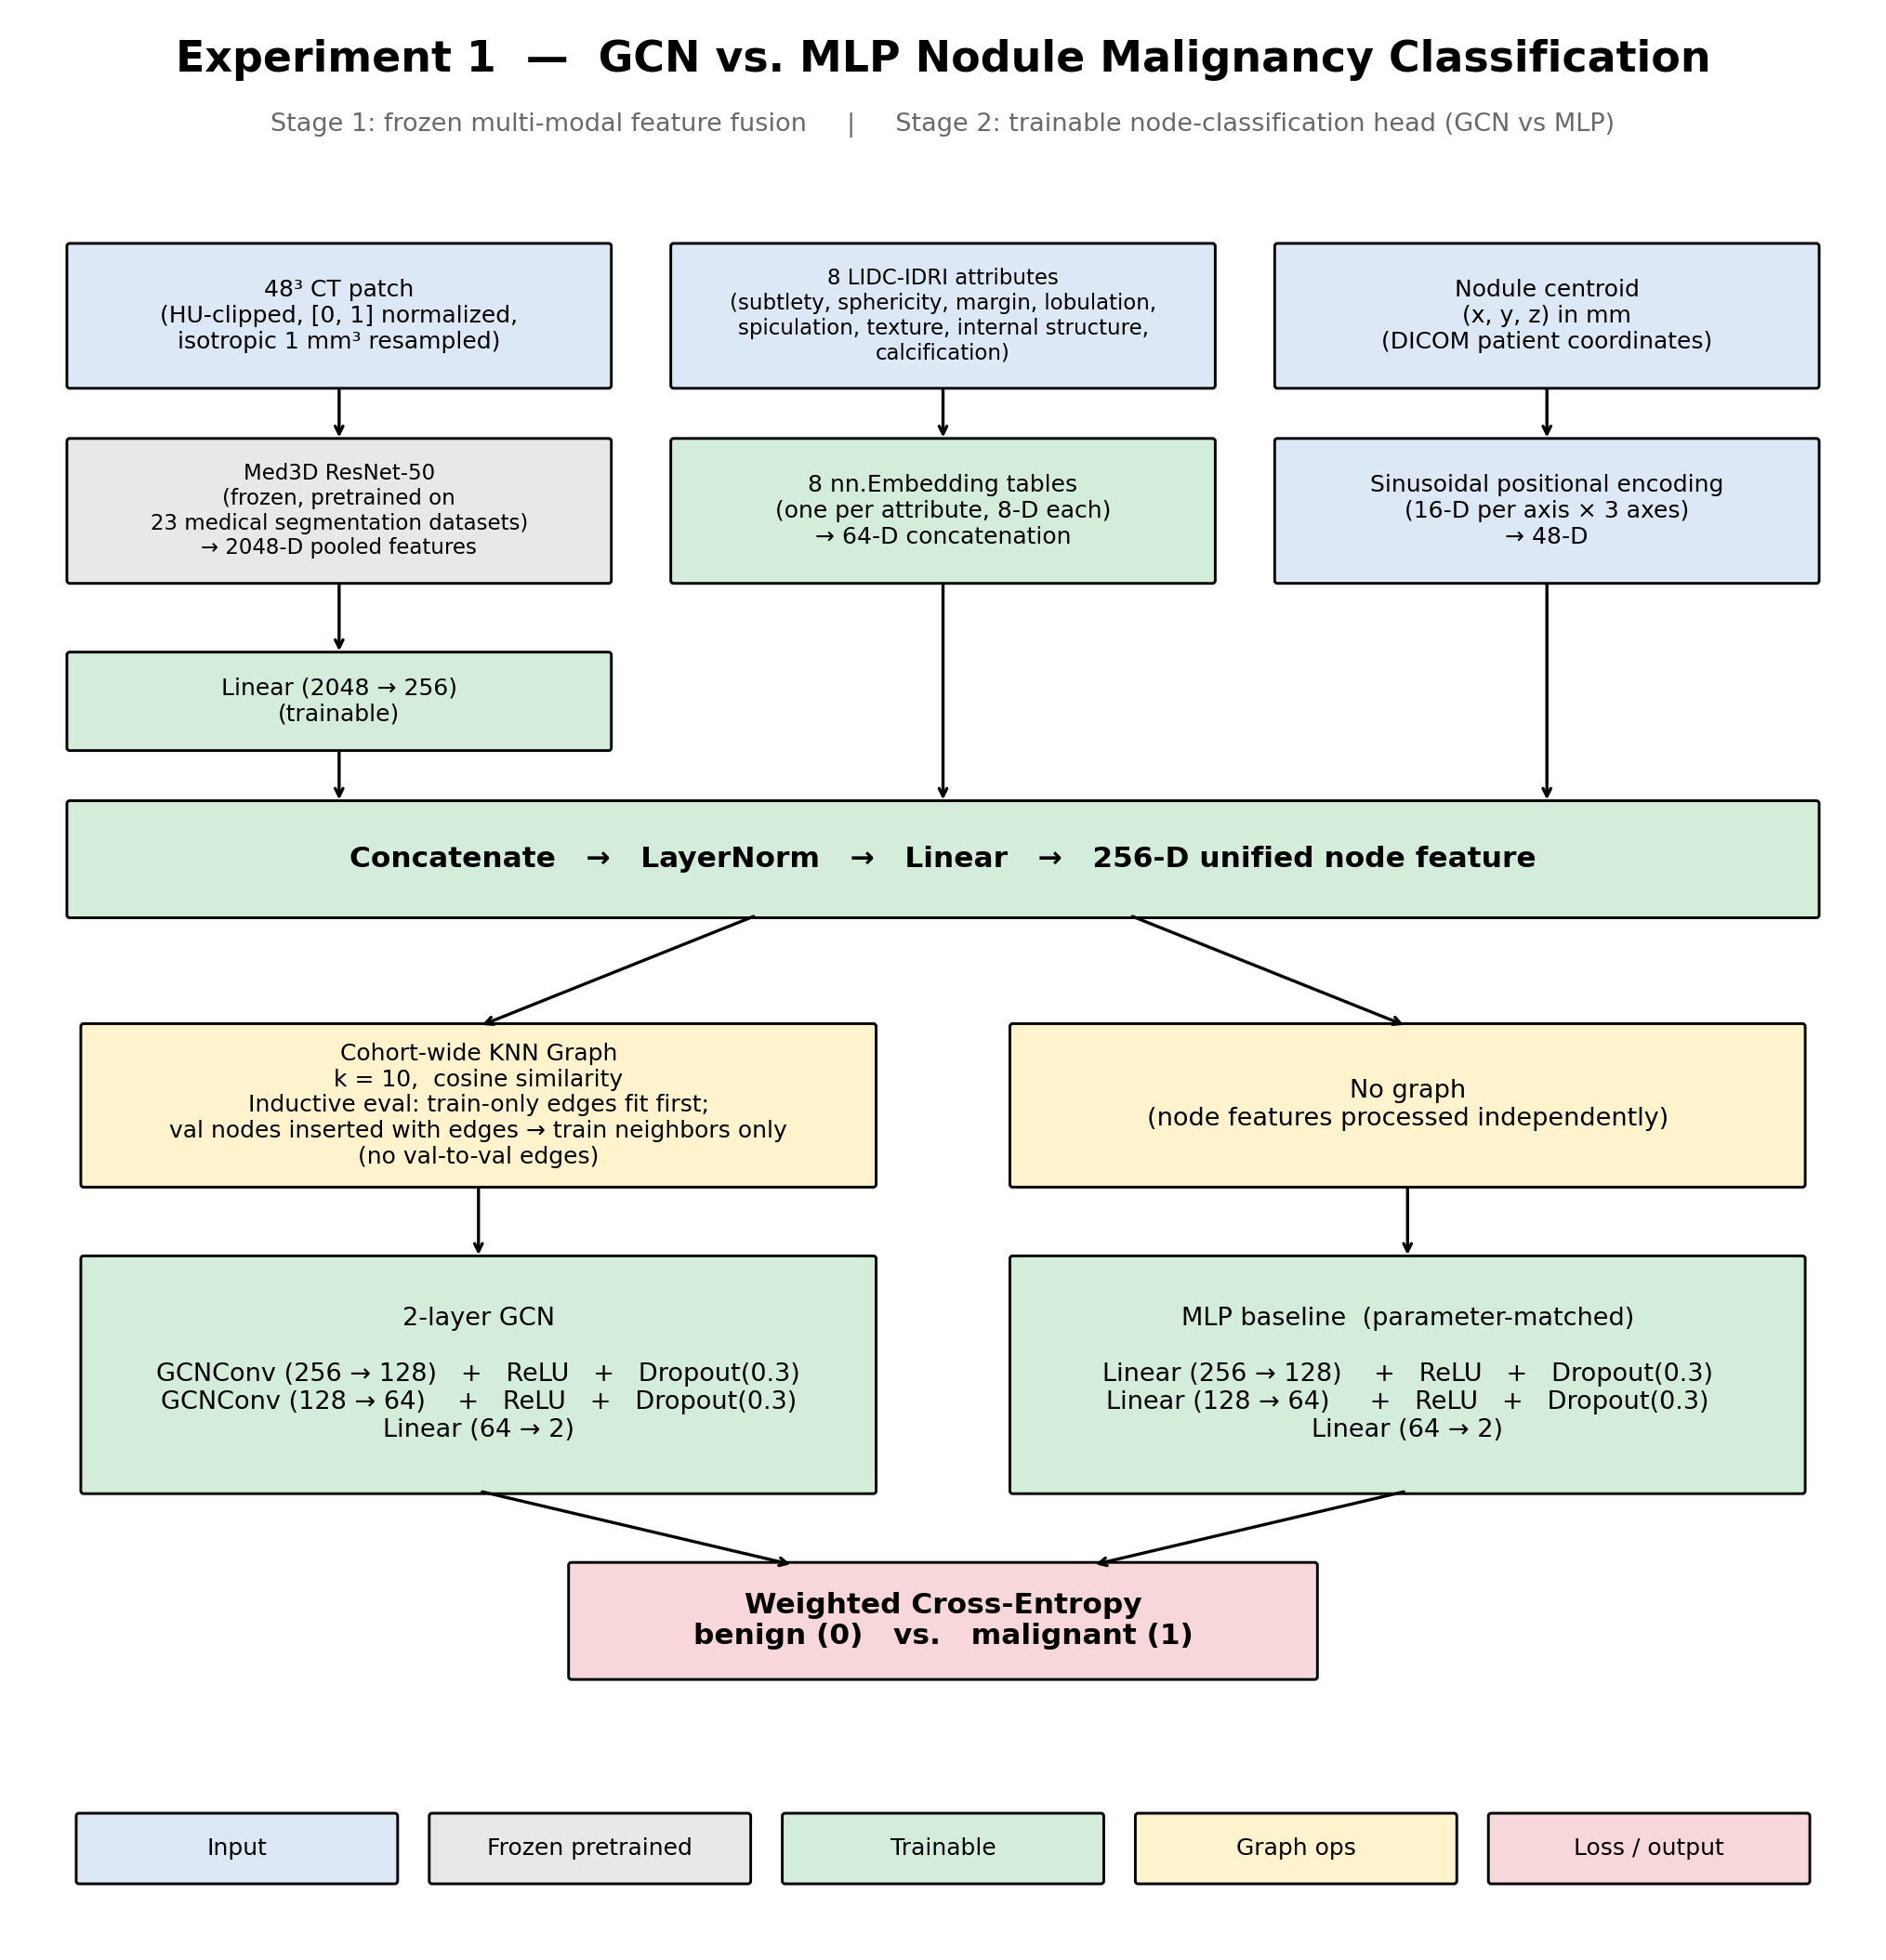
\includegraphics[width=0.7\linewidth]{image11.png}
\caption{Full pipeline diagram. Image, attribute, and spatial branches feed a 256-dimensional fused node representation, which is consumed by either the GCN head (treatment) or the parameter-matched MLP head (control).}
\label{fig:app-pipeline}
\end{figure}

\begin{figure}[h]
\centering
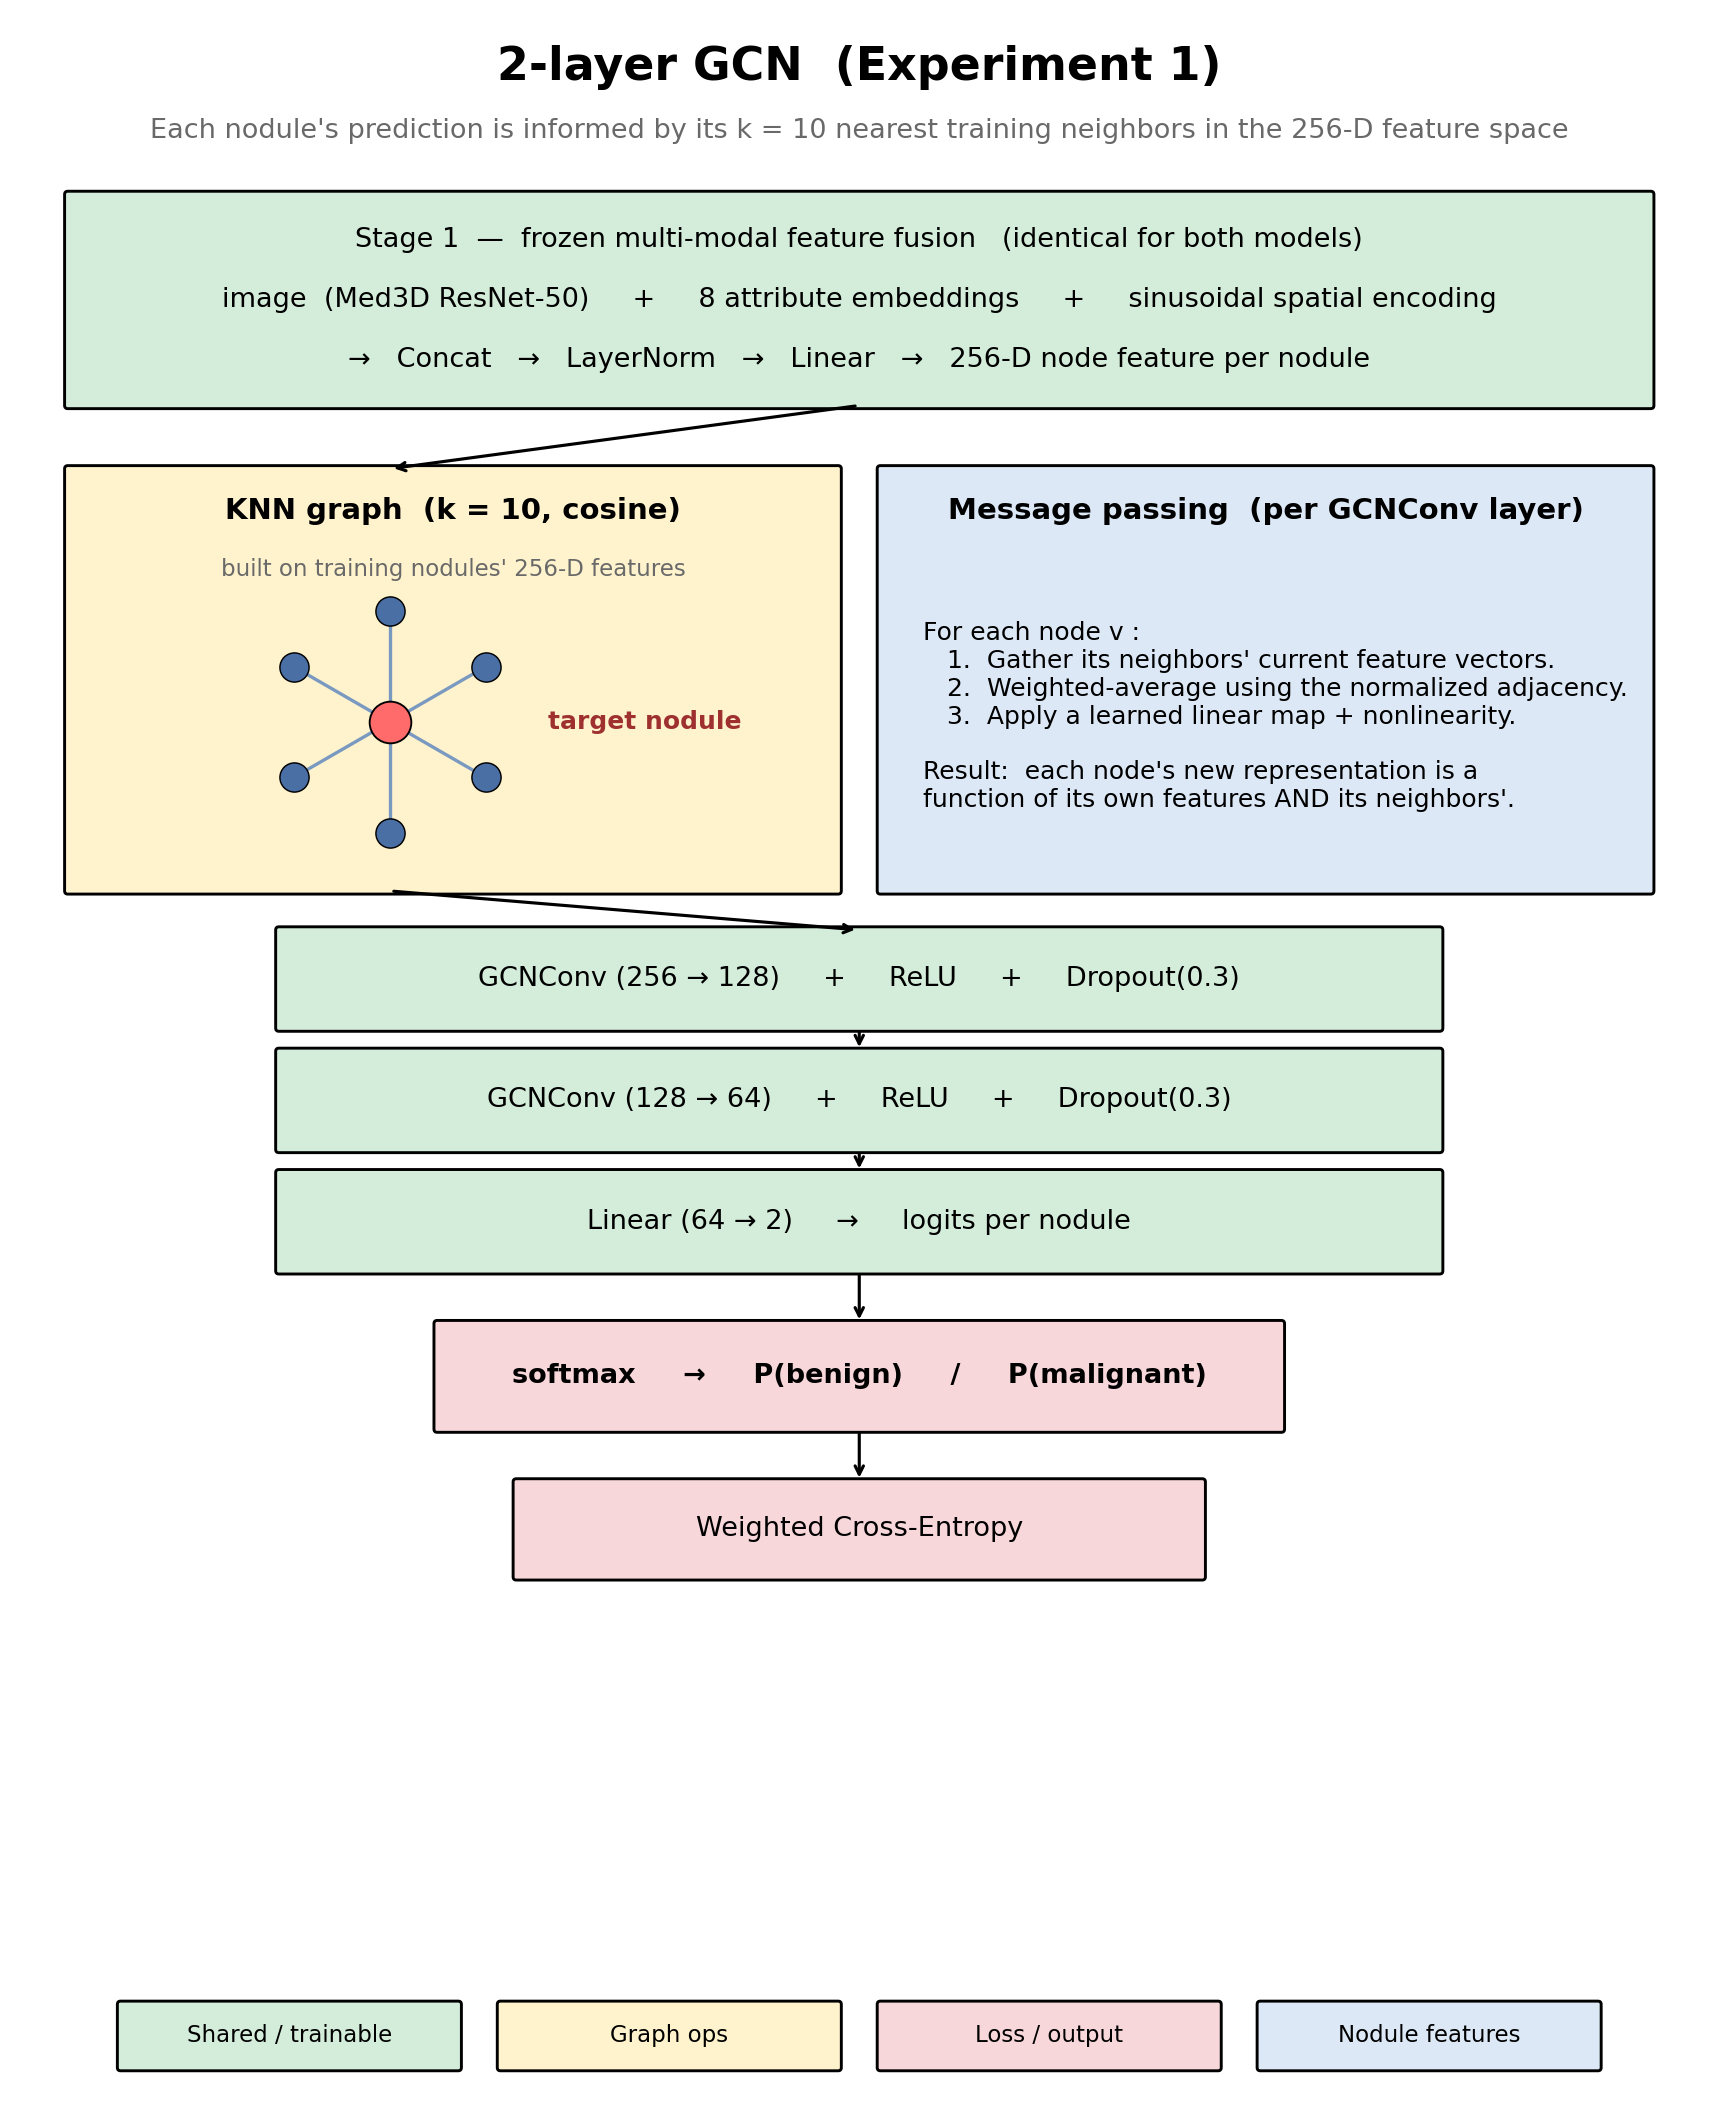
\includegraphics[width=0.7\linewidth]{image12.png}
\caption{GCN head detail. Two GCNConv layers operate over a cohort-wide $k$-nearest-neighbor graph in the 256-dimensional Stage-1 space. Symmetric normalization with self-loops, ReLU, and Dropout(0.3) are applied between layers, and a final linear layer maps to two class logits.}
\label{fig:app-gcn}
\end{figure}

\begin{figure}[h]
\centering
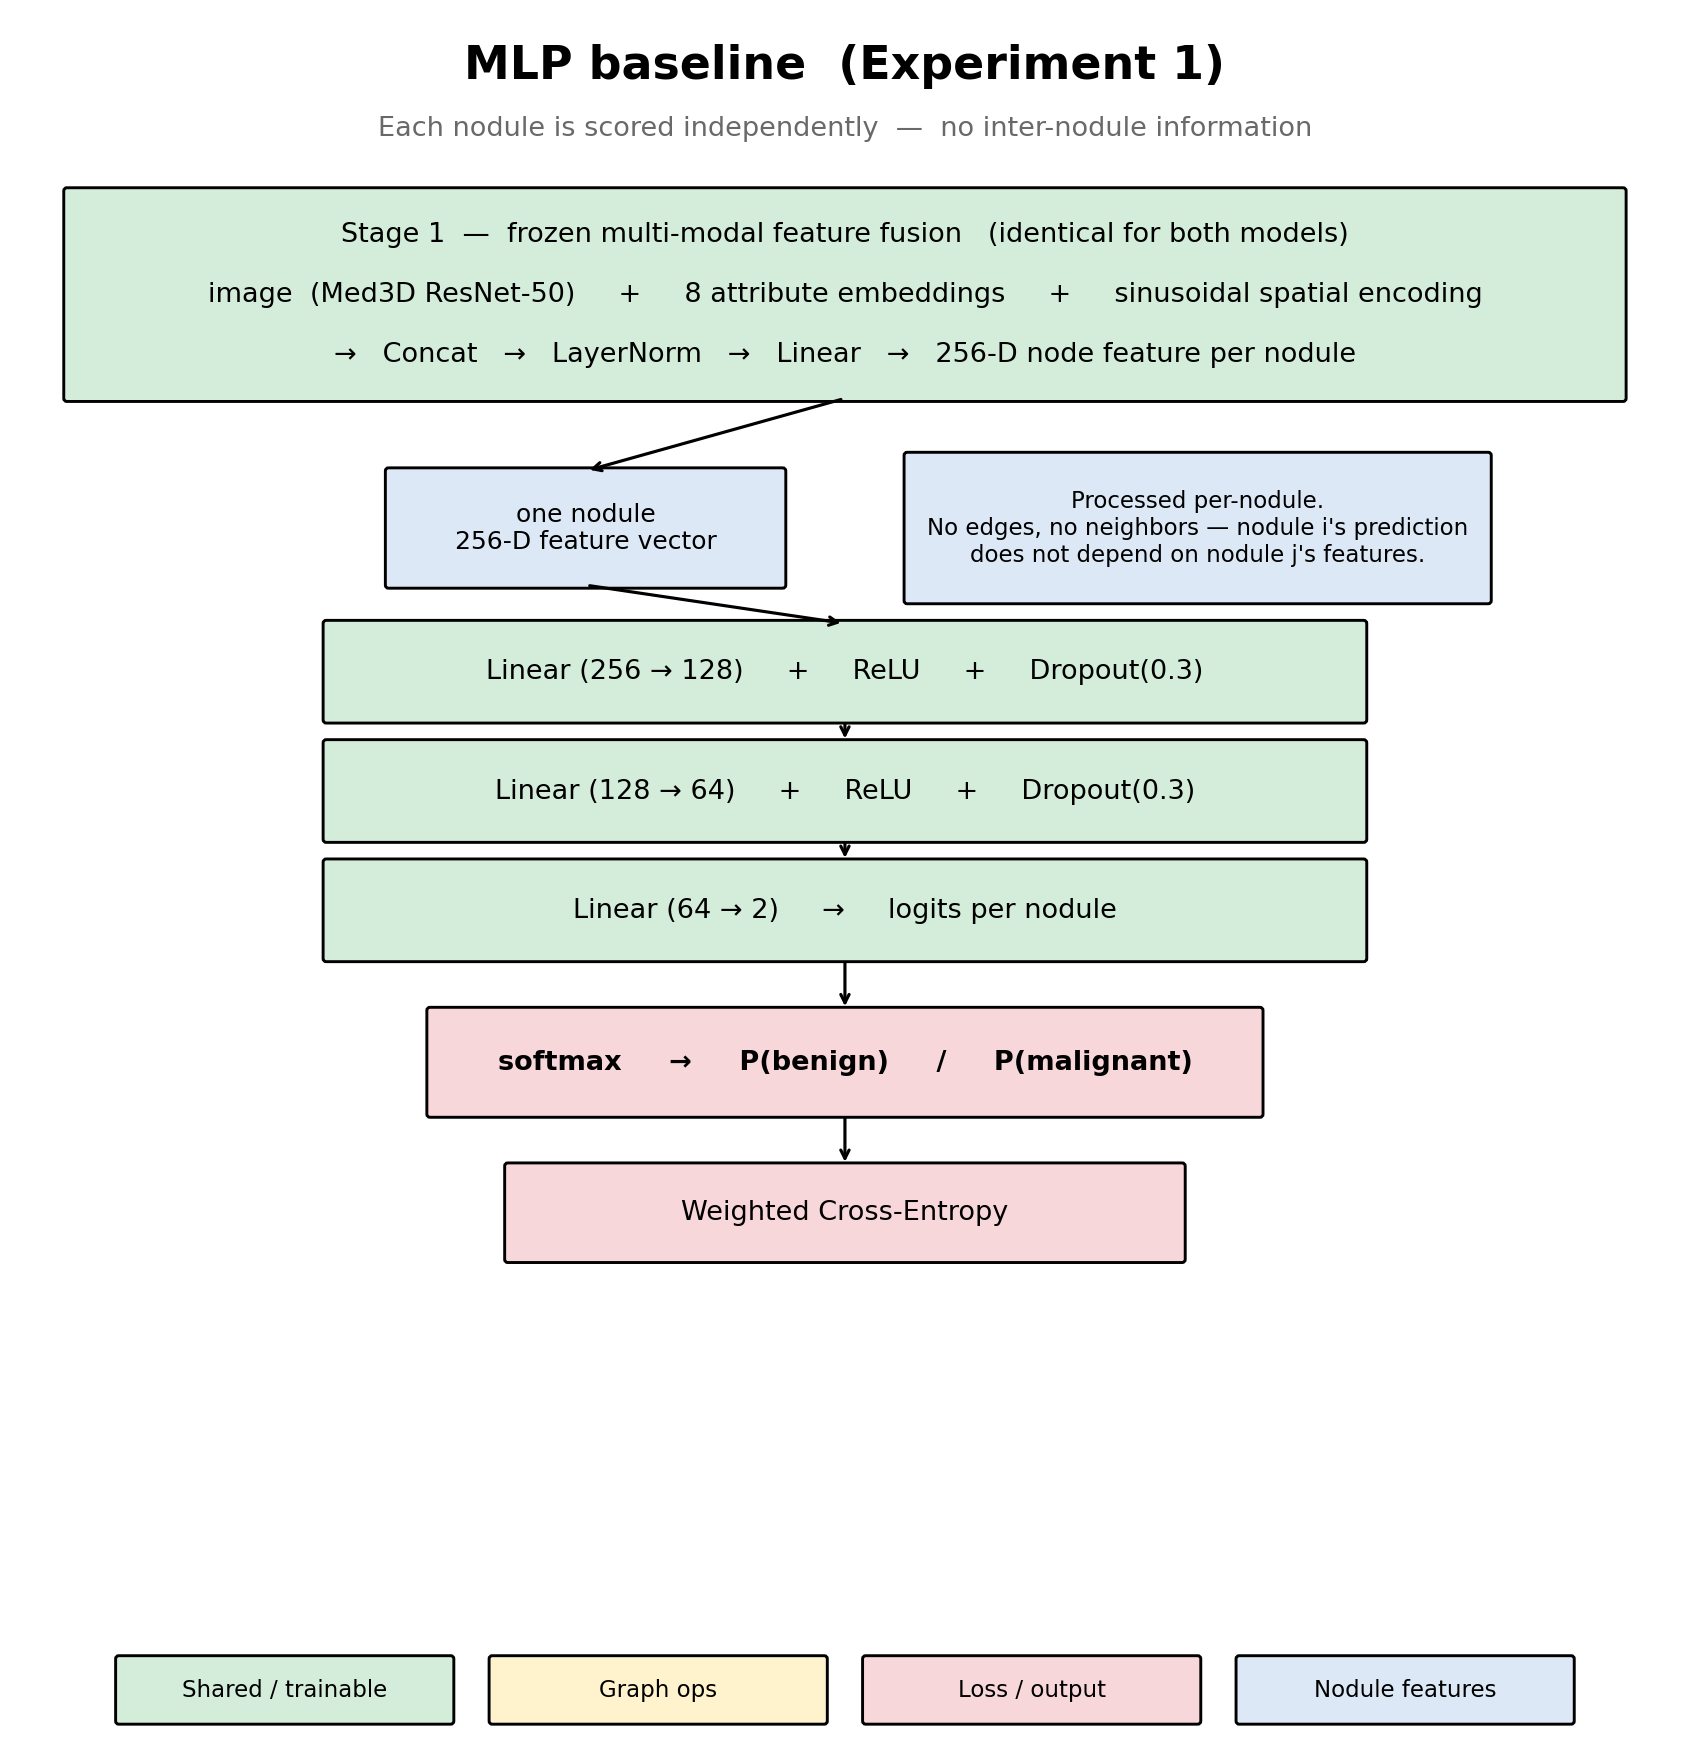
\includegraphics[width=0.7\linewidth]{image13.png}
\caption{MLP head detail. The MLP is parameter-matched to the GCN within $\pm 20\%$ of total parameters and shares all training hyperparameters; its key architectural difference is the absence of any graph structure, so each nodule is processed independently.}
\label{fig:app-mlp}
\end{figure}

\begin{figure}[h]
\centering
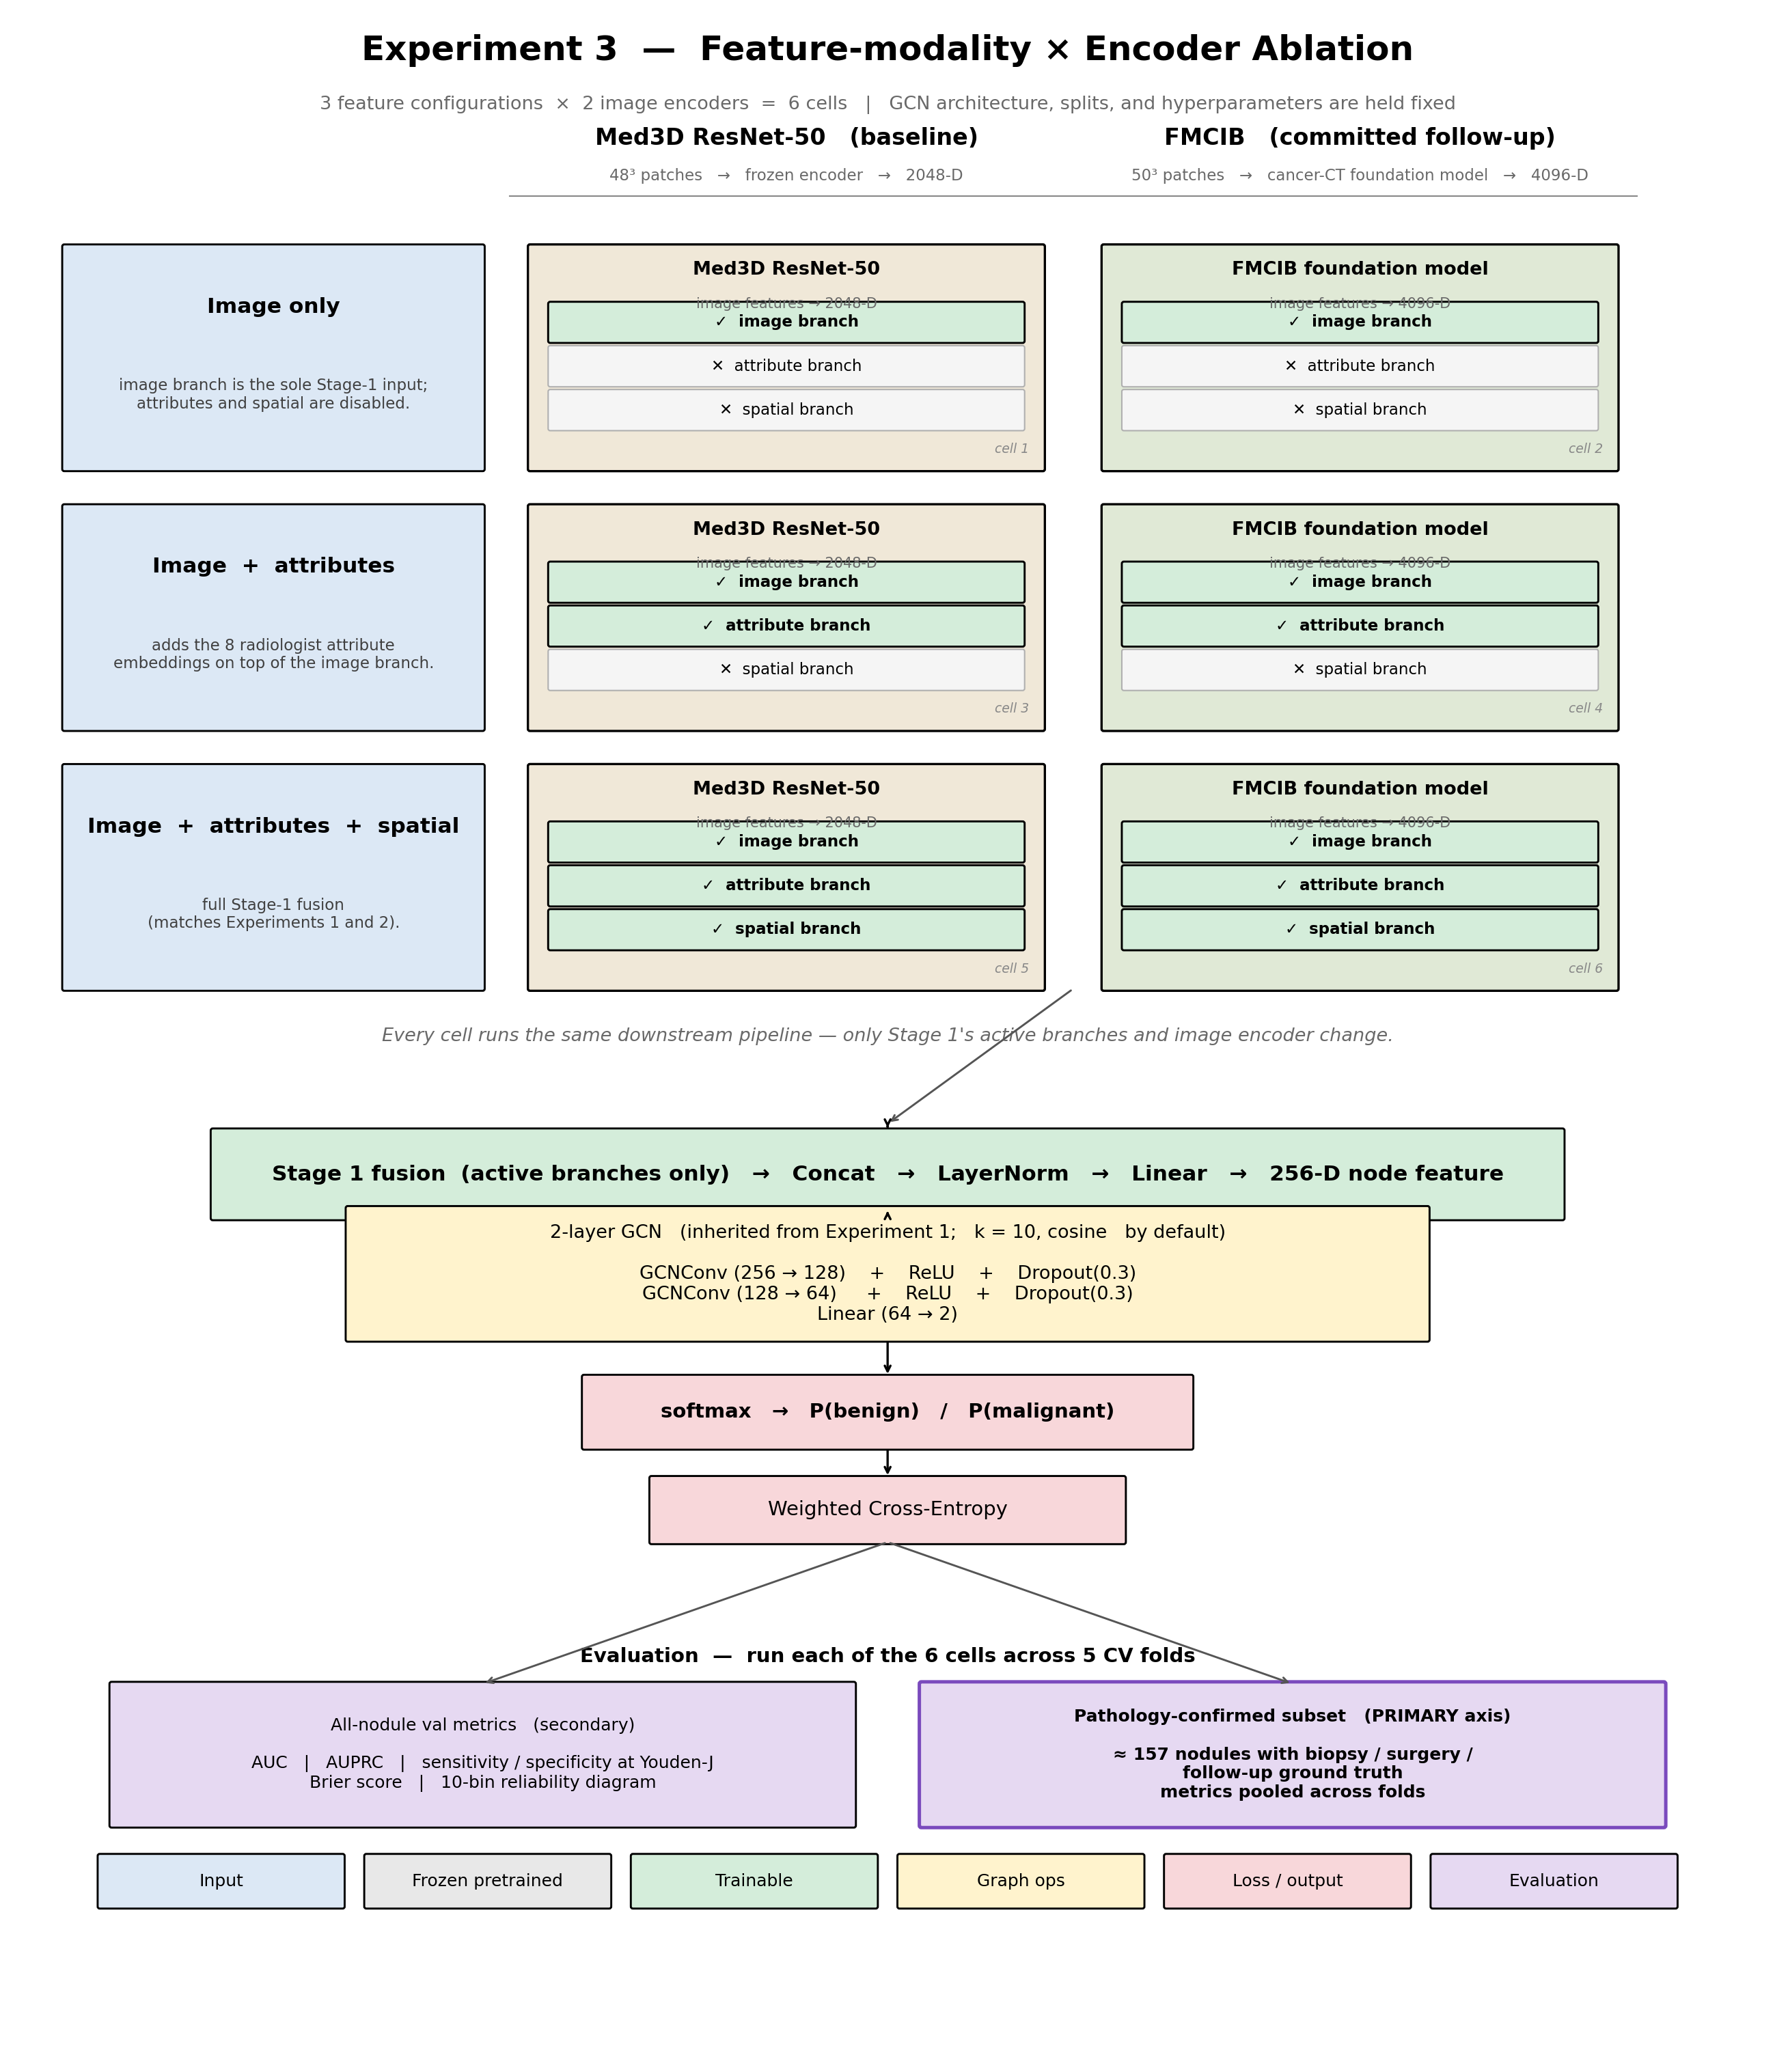
\includegraphics[width=0.7\linewidth]{image14.png}
\caption{Experiment-3 architectural grid. Three Stage-1 feature configurations (image only; image plus attributes; image plus attributes plus spatial) are crossed with two encoders (Med3D ResNet-50; FMCIB).}
\label{fig:app-exp3}
\end{figure}

\begin{figure}[h]
\centering
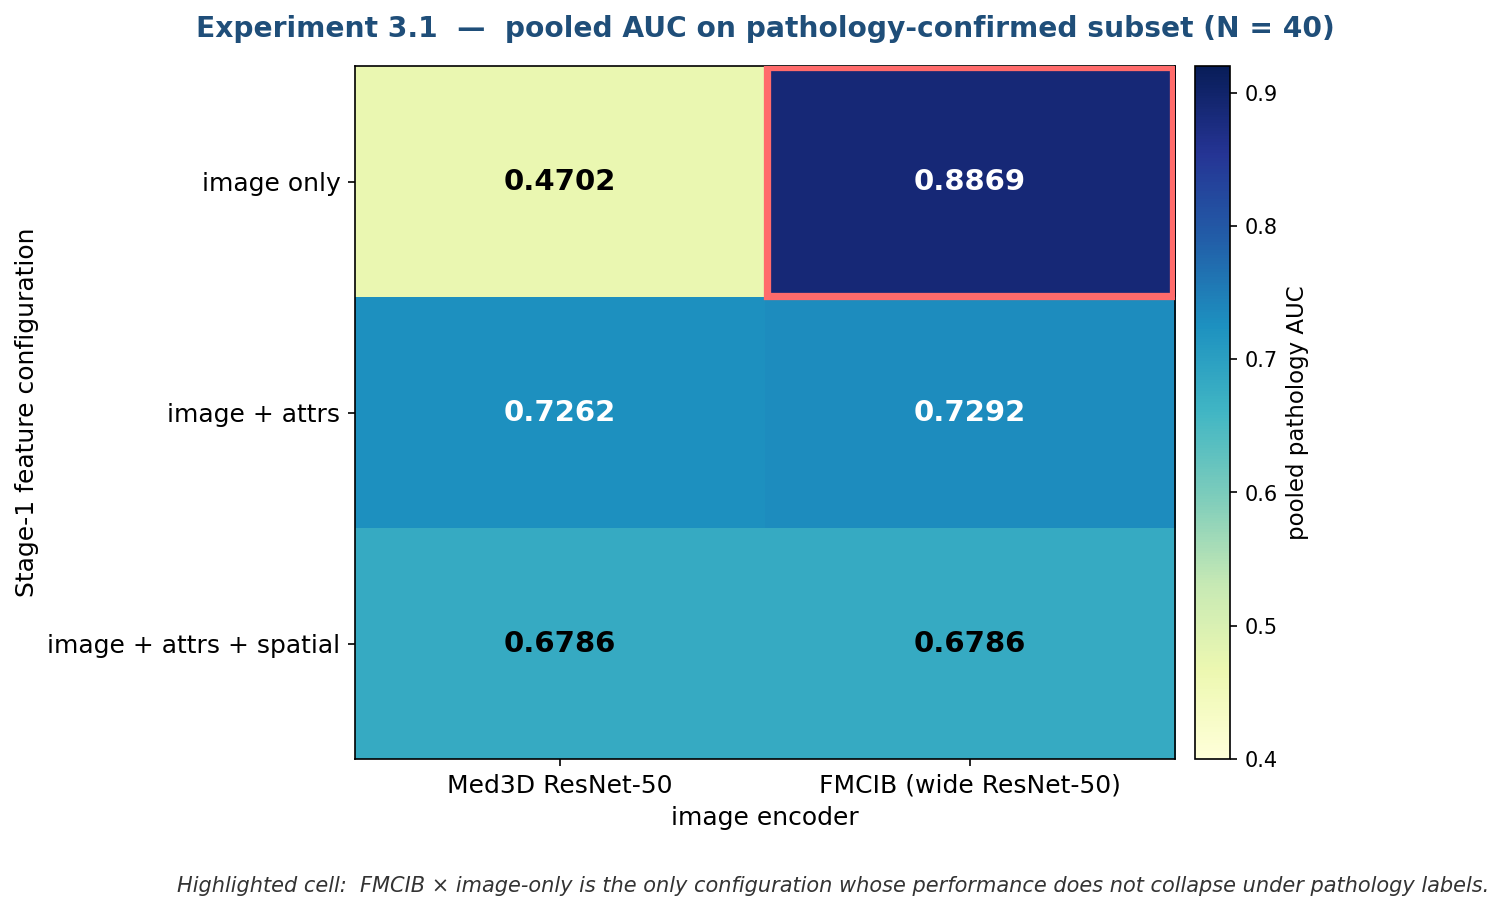
\includegraphics[width=0.85\linewidth]{image15.png}
\caption{Pooled pathology AUC heatmap ($N = 40$). The FMCIB image-only cell is highlighted as the only configuration whose performance does not collapse under pathology labels.}
\label{fig:app-path}
\end{figure}

\begin{figure}[h]
\centering
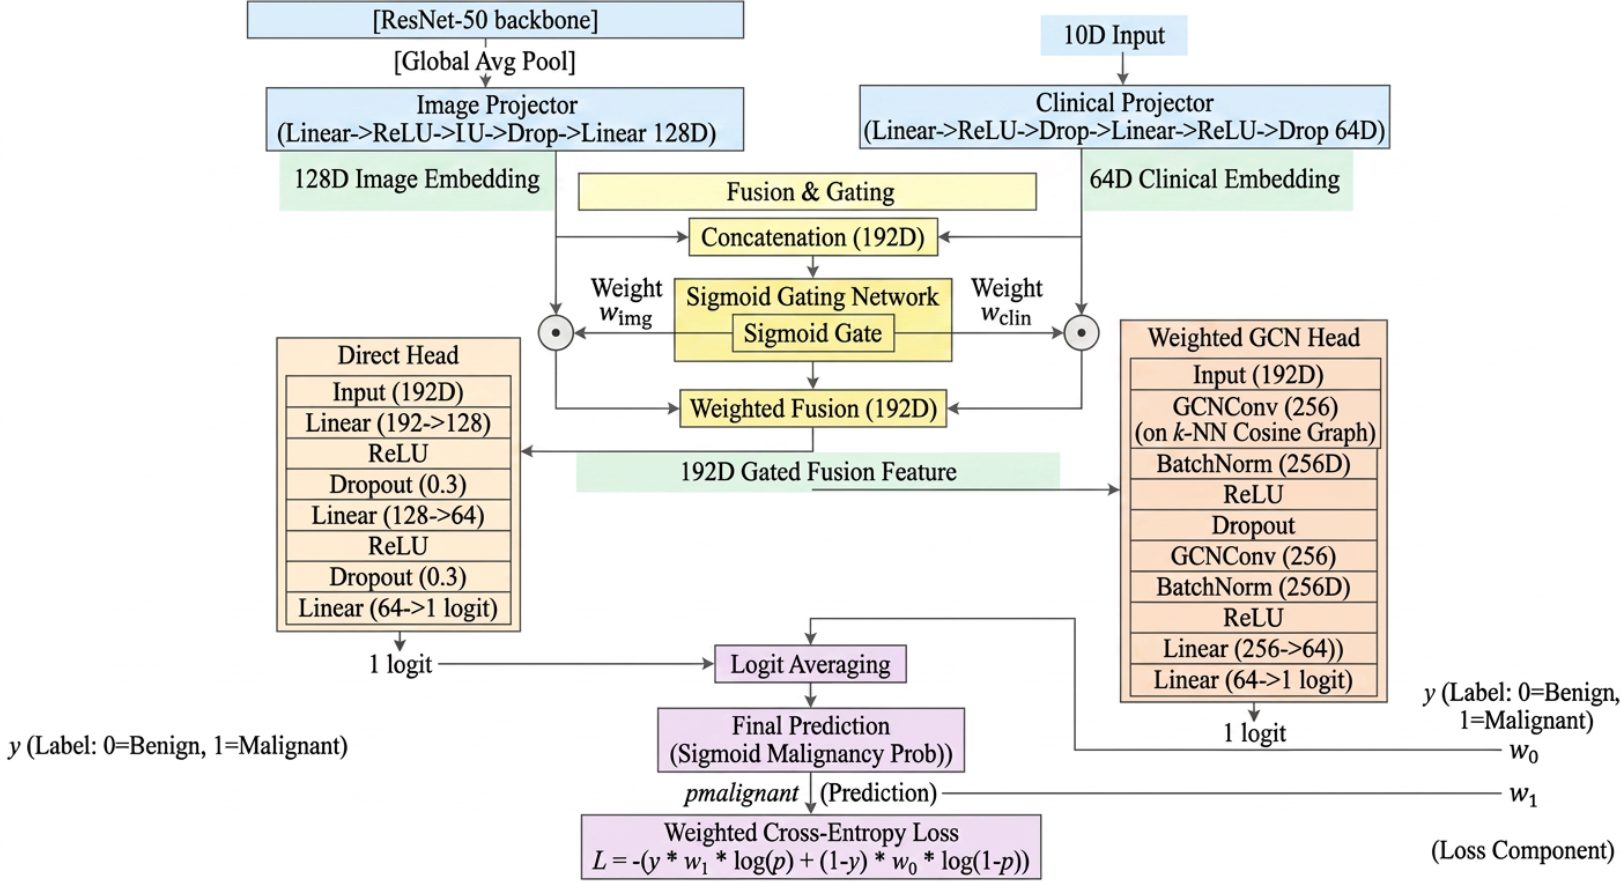
\includegraphics[width=0.85\linewidth]{image16.png}
\caption{Enhanced GCN model for handling the LIDC-IDRI dataset, which consists of both CT images and Radiomics features. This model achieved a highest of $99.17\%$ random validation accuracy and an all-time-highest validation accuracy of $97.71\%$ with ROC of $99.58$ in classification of cancer type.}
\label{fig:app-enhanced-gcn}
\end{figure}

\end{document}
